\documentclass[10pt, journal, letterpaper]{IEEEtran}
%\IEEEoverridecommandlockouts
% The preceding line is only needed to identify funding in the first footnote. If that is unneeded, please comment it out.
\usepackage{amsmath,amssymb,amsfonts}
\usepackage{algorithmic}
\usepackage{graphicx}
\usepackage{textcomp}
\usepackage{wrapfig}
\def\BibTeX{{\rm B\kern-.05em{\sc i\kern-.025em b}\kern-.08em
    T\kern-.1667em\lower.7ex\hbox{E}\kern-.125emX}}
%\markboth{\journalname, VOL. XX, NO. XX, XXXX 2017}
%{Author \MakeLowercase{\textit{et al.}}: Preparation of Papers for IEEE TRANSACTIONS and JOURNALS (February 2017)}
%\definecolor{abstractbg}{rgb}{0.89804,0.94510,0.83137}
%\setlength{\fboxrule}{0pt}
%\setlength{\fboxsep}{0pt}
\usepackage{float}
\usepackage{amsmath}
\usepackage{amssymb}
\usepackage{algorithmic}
\usepackage{graphicx}
\usepackage{textcomp}
\usepackage{xcolor}
\definecolor{subsectioncolor}{RGB}{0, 0, 255} % Defines subsectioncolor as blue
%multi line comments
\usepackage{verbatim }
% SI Unit Package
\usepackage{siunitx}

% Table Package
\usepackage{booktabs}
\usepackage{hyperref}
\usepackage{balance}
\usepackage{url}
\usepackage{tabularx}
\usepackage{array}
%bib package 

\usepackage{scalerel}
\usepackage{tikz}
\usetikzlibrary{svg.path}
\definecolor{orcidlogocol}{HTML}{A6CE39}
\tikzset{
  orcidlogo/.pic={
    \fill[orcidlogocol] svg{M256,128c0,70.7-57.3,128-128,128C57.3,256,0,198.7,0,128C0,57.3,57.3,0,128,0C198.7,0,256,57.3,256,128z};
    \fill[white] svg{M86.3,186.2H70.9V79.1h15.4v48.4V186.2z}
                 svg{M108.9,79.1h41.6c39.6,0,57,28.3,57,53.6c0,27.5-21.5,53.6-56.8,53.6h-41.8V79.1z M124.3,172.4h24.5c34.9,0,42.9-26.5,42.9-39.7c0-21.5-13.7-39.7-43.7-39.7h-23.7V172.4z}
                 svg{M88.7,56.8c0,5.5-4.5,10.1-10.1,10.1c-5.6,0-10.1-4.6-10.1-10.1c0-5.6,4.5-10.1,10.1-10.1C84.2,46.7,88.7,51.3,88.7,56.8z};
  }
}
\newcommand\orcidicon[1]{\href{https://orcid.org/#1}{\mbox{\scalerel*{

\begin{tikzpicture}[yscale=-1,transform shape]
\pic{orcidlogo};
\end{tikzpicture}
}{|}}}}

%Image Package
\usepackage{svg}

\begin{document}
\title{
Prediction of the Received Power of Low-Power Networks Using Inertial Sensors
}

\author{Waltenegus Dargie\orcidicon{0000-0002-7911-8081}, \IEEEmembership{Senior Member, IEEE}, Christian Poellabauer\orcidicon{0000-0002-0599-7941}, \IEEEmembership{Senior Member, IEEE}, and Abiy Tasissa\orcidicon{0000-0003-4033-7735}  
    \thanks{Manuscript submitted on 1 January 2025.}
    \thanks{This work has been partially funded by the German Research Foundation (DFG) under project agreements DA 1211/7-1 and NSF DMS 2208392}
    \thanks{W. Dargie is with the Faculty of Computer Science, Technische Universit{\"a}t Dresden, 01062 Dresden, Germany (e-mail: waltenegus.dargie@tu-dresden.de)}
    \thanks{C. Poellabauer is with the Knight Foundation School of Computing and Information Sciences at Florida International University, USA, (e-mail:  cpoellab@fiu.edu)}
    \thanks{A. Tasissa is with the Department of Mathematics, Tufts University, USA (Abiy.Tasissa@tufts.edu)} 
}
\maketitle

\begin{abstract}
Low-power and cost-effective IoT sensing nodes enable scalable monitoring of different environments. Some of these environments impose rough and extreme operating conditions, requiring  continuous adaptation and reconfiguration of physical and link layer parameters. In this paper, we closely investigate the stability of the wireless links established between nodes deployed on the surface of different water bodies and propose a model to predict the received power. Our model is based on Minimum Mean Square Estimation (MMSE) and relies on the statistics of received power and the motion the nodes experience during communication. One of the drawbacks of MMSE is its reliance on matrix inversion, which is at once computationally expensive and difficult to implement with resource constrained devices. We forgo this stage by estimating model parameters using the gradient-descent approach, which is much simpler to implement. The model achieves a prediction accuracy of 91\% even with a small number of iterations and a significant amount of water motion during communication.
\end{abstract}

%%
%% The code below is generated by the tool at http://dl.acm.org/ccs.cfm.
%% Please copy and paste the code instead of the example below.
%%


%%
%% Keywords. The author(s) should pick words that accurately describe
%% the work being presented. Separate the keywords with commas.
\begin{IEEEkeywords}
Adaptive transmission power, Inertial Measurement Unit (IMU), wireless sensor networks, link quality estimation, water quality monitoring, Internet-of-Things 
\end{IEEEkeywords}

%% A "teaser" image appears between the author and affiliation
%% information and the body of the document, and typically spans the
%% page.
%%
%% This command processes the author and affiliation and title
%% information and builds the first part of the formatted document.

\section{Introduction}


\begin{figure}[t]
\centering
\includegraphics[width=0.6\columnwidth]{figures/evaluation_desiderata_V5.pdf}
\vspace{-0.5cm}
\caption{\systemName is a platform for conducting realistic evaluations of code LLMs, collecting human preferences of coding models with real users, real tasks, and in realistic environments, aimed at addressing the limitations of existing evaluations.
}
\label{fig:motivation}
\end{figure}

\begin{figure*}[t]
\centering
\includegraphics[width=\textwidth]{figures/system_design_v2.png}
\caption{We introduce \systemName, a VSCode extension to collect human preferences of code directly in a developer's IDE. \systemName enables developers to use code completions from various models. The system comprises a) the interface in the user's IDE which presents paired completions to users (left), b) a sampling strategy that picks model pairs to reduce latency (right, top), and c) a prompting scheme that allows diverse LLMs to perform code completions with high fidelity.
Users can select between the top completion (green box) using \texttt{tab} or the bottom completion (blue box) using \texttt{shift+tab}.}
\label{fig:overview}
\end{figure*}

As model capabilities improve, large language models (LLMs) are increasingly integrated into user environments and workflows.
For example, software developers code with AI in integrated developer environments (IDEs)~\citep{peng2023impact}, doctors rely on notes generated through ambient listening~\citep{oberst2024science}, and lawyers consider case evidence identified by electronic discovery systems~\citep{yang2024beyond}.
Increasing deployment of models in productivity tools demands evaluation that more closely reflects real-world circumstances~\citep{hutchinson2022evaluation, saxon2024benchmarks, kapoor2024ai}.
While newer benchmarks and live platforms incorporate human feedback to capture real-world usage, they almost exclusively focus on evaluating LLMs in chat conversations~\citep{zheng2023judging,dubois2023alpacafarm,chiang2024chatbot, kirk2024the}.
Model evaluation must move beyond chat-based interactions and into specialized user environments.



 

In this work, we focus on evaluating LLM-based coding assistants. 
Despite the popularity of these tools---millions of developers use Github Copilot~\citep{Copilot}---existing
evaluations of the coding capabilities of new models exhibit multiple limitations (Figure~\ref{fig:motivation}, bottom).
Traditional ML benchmarks evaluate LLM capabilities by measuring how well a model can complete static, interview-style coding tasks~\citep{chen2021evaluating,austin2021program,jain2024livecodebench, white2024livebench} and lack \emph{real users}. 
User studies recruit real users to evaluate the effectiveness of LLMs as coding assistants, but are often limited to simple programming tasks as opposed to \emph{real tasks}~\citep{vaithilingam2022expectation,ross2023programmer, mozannar2024realhumaneval}.
Recent efforts to collect human feedback such as Chatbot Arena~\citep{chiang2024chatbot} are still removed from a \emph{realistic environment}, resulting in users and data that deviate from typical software development processes.
We introduce \systemName to address these limitations (Figure~\ref{fig:motivation}, top), and we describe our three main contributions below.


\textbf{We deploy \systemName in-the-wild to collect human preferences on code.} 
\systemName is a Visual Studio Code extension, collecting preferences directly in a developer's IDE within their actual workflow (Figure~\ref{fig:overview}).
\systemName provides developers with code completions, akin to the type of support provided by Github Copilot~\citep{Copilot}. 
Over the past 3 months, \systemName has served over~\completions suggestions from 10 state-of-the-art LLMs, 
gathering \sampleCount~votes from \userCount~users.
To collect user preferences,
\systemName presents a novel interface that shows users paired code completions from two different LLMs, which are determined based on a sampling strategy that aims to 
mitigate latency while preserving coverage across model comparisons.
Additionally, we devise a prompting scheme that allows a diverse set of models to perform code completions with high fidelity.
See Section~\ref{sec:system} and Section~\ref{sec:deployment} for details about system design and deployment respectively.



\textbf{We construct a leaderboard of user preferences and find notable differences from existing static benchmarks and human preference leaderboards.}
In general, we observe that smaller models seem to overperform in static benchmarks compared to our leaderboard, while performance among larger models is mixed (Section~\ref{sec:leaderboard_calculation}).
We attribute these differences to the fact that \systemName is exposed to users and tasks that differ drastically from code evaluations in the past. 
Our data spans 103 programming languages and 24 natural languages as well as a variety of real-world applications and code structures, while static benchmarks tend to focus on a specific programming and natural language and task (e.g. coding competition problems).
Additionally, while all of \systemName interactions contain code contexts and the majority involve infilling tasks, a much smaller fraction of Chatbot Arena's coding tasks contain code context, with infilling tasks appearing even more rarely. 
We analyze our data in depth in Section~\ref{subsec:comparison}.



\textbf{We derive new insights into user preferences of code by analyzing \systemName's diverse and distinct data distribution.}
We compare user preferences across different stratifications of input data (e.g., common versus rare languages) and observe which affect observed preferences most (Section~\ref{sec:analysis}).
For example, while user preferences stay relatively consistent across various programming languages, they differ drastically between different task categories (e.g. frontend/backend versus algorithm design).
We also observe variations in user preference due to different features related to code structure 
(e.g., context length and completion patterns).
We open-source \systemName and release a curated subset of code contexts.
Altogether, our results highlight the necessity of model evaluation in realistic and domain-specific settings.





\putsec{related}{Related Work}

\noindent \textbf{Efficient Radiance Field Rendering.}
%
The introduction of Neural Radiance Fields (NeRF)~\cite{mil:sri20} has
generated significant interest in efficient 3D scene representation and
rendering for radiance fields.
%
Over the past years, there has been a large amount of research aimed at
accelerating NeRFs through algorithmic or software
optimizations~\cite{mul:eva22,fri:yu22,che:fun23,sun:sun22}, and the
development of hardware
accelerators~\cite{lee:cho23,li:li23,son:wen23,mub:kan23,fen:liu24}.
%
The state-of-the-art method, 3D Gaussian splatting~\cite{ker:kop23}, has
further fueled interest in accelerating radiance field
rendering~\cite{rad:ste24,lee:lee24,nie:stu24,lee:rho24,ham:mel24} as it
employs rasterization primitives that can be rendered much faster than NeRFs.
%
However, previous research focused on software graphics rendering on
programmable cores or building dedicated hardware accelerators. In contrast,
\name{} investigates the potential of efficient radiance field rendering while
utilizing fixed-function units in graphics hardware.
%
To our knowledge, this is the first work that assesses the performance
implications of rendering Gaussian-based radiance fields on the hardware
graphics pipeline with software and hardware optimizations.

%%%%%%%%%%%%%%%%%%%%%%%%%%%%%%%%%%%%%%%%%%%%%%%%%%%%%%%%%%%%%%%%%%%%%%%%%%
\myparagraph{Enhancing Graphics Rendering Hardware.}
%
The performance advantage of executing graphics rendering on either
programmable shader cores or fixed-function units varies depending on the
rendering methods and hardware designs.
%
Previous studies have explored the performance implication of graphics hardware
design by developing simulation infrastructures for graphics
workloads~\cite{bar:gon06,gub:aam19,tin:sax23,arn:par13}.
%
Additionally, several studies have aimed to improve the performance of
special-purpose hardware such as ray tracing units in graphics
hardware~\cite{cho:now23,liu:cha21} and proposed hardware accelerators for
graphics applications~\cite{lu:hua17,ram:gri09}.
%
In contrast to these works, which primarily evaluate traditional graphics
workloads, our work focuses on improving the performance of volume rendering
workloads, such as Gaussian splatting, which require blending a huge number of
fragments per pixel.

%%%%%%%%%%%%%%%%%%%%%%%%%%%%%%%%%%%%%%%%%%%%%%%%%%%%%%%%%%%%%%%%%%%%%%%%%%
%
In the context of multi-sample anti-aliasing, prior work proposed reducing the
amount of redundant shading by merging fragments from adjacent triangles in a
mesh at the quad granularity~\cite{fat:bou10}.
%
While both our work and quad-fragment merging (QFM)~\cite{fat:bou10} aim to
reduce operations by merging quads, our proposed technique differs from QFM in
many aspects.
%
Our method aims to blend \emph{overlapping primitives} along the depth
direction and applies to quads from any primitive. In contrast, QFM merges quad
fragments from small (e.g., pixel-sized) triangles that \emph{share} an edge
(i.e., \emph{connected}, \emph{non-overlapping} triangles).
%
As such, QFM is not applicable to the scenes consisting of a number of
unconnected transparent triangles, such as those in 3D Gaussian splatting.
%
In addition, our method computes the \emph{exact} color for each pixel by
offloading blending operations from ROPs to shader units, whereas QFM
\emph{approximates} pixel colors by using the color from one triangle when
multiple triangles are merged into a single quad.


\section{Deployment}
\label{section:deployment}

\subsection{RecSys use case}\label{section:recsys-deploy}
SLM variants of the RecSys use case have been deployed to an A/B test.

\noindent \textbf{Serving Infrastructure} For all use cases, we benchmark and serve traffic using nodes with 256 CPU cores, 2TB of host memory and 8 NVIDIA H100 GPUs. As mentioned earlier, we deploy SGLang (version 0.4.1) as the serving engine. We use tensor parallelism to concurrently use more than 1 GPU for inference. To maximize performance, we employ FP8 quantization for both weights and activations and use FlashInfer~\cite{ye2025flashinfer} as the primary attention backend. Moreover, SGLang incorporates RadixAttention, which enables prefix caching for prompts sharing common prefixes.

\noindent \textbf{Workloads} For the RecSys workload, we follow the prompt structure outlined in Section~\ref{subsection:recsys_task} and utilize context lengths of 16k and 32k. Given the predictive nature of the task, the output length (i.e., the number of generated tokens) is set to 1, rendering the workload heavily reliant on the prefill phase. Consequently, optimizing the prefill stage is crucial for performance. For instance, prefix caching substantially improves prefill (and decode) times when a prompt’s key (K) and value (V) tensors for its shared prefix have already been processed. In cases where there are $k$ candidate items to be ranked for a member $m$, $k$ prompts are served. These prompts share a long prefix containing the user information and historical item interactions. Once one prompt is served, its KV tensors are cached, allowing subsequent prompts for the same member to reuse the cached data—a process we refer to as a hot prefill.

\noindent \textbf{Metrics} We use two key metrics - time to first token (TTFT) and time per output token (TPOT). For prediction tasks, which are prefill-intensive, TTFT is the primary metric as it reflects the duration of the prefill phase. For generative tasks, both TTFT and TPOT are important. Additionally, we report the total serving throughput for various context lengths.

\noindent \textbf{Results} In terms of quality, the models under consideration performn similarly since their AUCs are similar. For performance, we report TTFT and throughput measurements for both 16k and 32k context lengths. P99 TTFT results for a workload with 1 QPS (i.e., $m=1$) and 1 or more prompt per member (i.e., $k=1$ or more) can be found in Figure~\ref{figure:p99ttft} (detailed p50, p99 and throughput numbers can be found in Tables~\ref{table:m1k1_16k}, ~\ref{table:m1k1_32k} and ~\ref{table:m1k4_32k} in Appendix~\ref{subsec:Extra tables}). From the figure and the tables, we can conclude that latency drops drastically as model size becomes smaller. Serving traffic with 32k context is significantly slower than serving traffic with 16k context. Setting $k$ more than 1 doesn't hurt latency much, because of KV caching. 

To better understand the effect of model pruning on inference latency, we present the break down of forward pass for a single layer in Figure~\ref{figure:profiling}. As it can be seen, the attention step is the main latency bottleneck. Our structured pruning of the attention heads improves the attention latency by about $40\%$ which in turn results in more than $28\%$ speed up in prefill latency.



\begin{figure}[htbp]
  \centering
  \begin{tikzpicture}
    \begin{axis}[
      xlabel={LLMs},
      ylabel={P99 TTFT (ms)},
      xlabel style={font=\large},
      ylabel style={font=\large},
      xtick=data,                    
      symbolic x coords={FM,8B,6.4B,3B,2.4B,2.1B},
      x tick label style={rotate=45, anchor=east},
      width=0.9\columnwidth,        
      height=0.7\columnwidth,       
      legend style={at={(0.95,0.95)}, anchor=north east} 
    ]
      \addplot[
        mark=*,
        color=myblue,
        thick,
        nodes near coords={\pgfkeysvalueof{/pgfplots/y}},
        every node near coord/.append style={font=\footnotesize, anchor=south}
      ] coordinates {
        (8B,282)
        (6.4B,262)
        (3B,209)
        (2.4B,197)
        (2.1B,184)
      };
      \addlegendentry{m=1, k=1, 16k};

      \addplot[
        mark=square*,
        color=myorange,
        thick,
        nodes near coords={\pgfkeysvalueof{/pgfplots/y}},
        every node near coord/.append style={font=\footnotesize, anchor=south}
      ] coordinates {
        (8B,643)
        (6.4B,613)
        (3B,472)
        (2.4B,456)
        (2.1B,391)
      };
      \addlegendentry{m=1, k=1, 32k};

      \addplot[
        mark=triangle*,
        color=mygreen,
        thick,
        nodes near coords={\pgfkeysvalueof{/pgfplots/y}},
        every node near coord/.append style={font=\footnotesize, anchor=south}
      ] coordinates {
        (8B,671)
        (6.4B,655)
        (3B,500)
        (2.4B,488)
        (2.1B,403)
      };
      \addlegendentry{m=1, k=4, 32k};

    \end{axis}
  \end{tikzpicture}
  \caption{P99 TTFT (ms) for various LLMs}
  \label{figure:p99ttft}
\end{figure}




\subsection{Generative use case}

\begin{table}[t]

\centering
\begin{tabular}{lc}
\hline\hline
\textbf{Model} & \textbf{IQM (\%)} \\
\hline\hline
KD Model   &+20.29\%  \\
\hline\hline
\end{tabular}
\caption{Online A/B test results for reasoning task.}
\label{table:gen_use_case_online}
\label{tab:gen_use_case_online}
\end{table}%

The reasoning task outlined in Section 4.3 was launched online for a 1\% A/B test. Results are outlined in Table~\ref{tab:gen_use_case_online}. KD, along with data changes, helped the model improve by 20.29\% on an internal quality metric (IQM). We also discuss deployment lessons from a generative use case to study the effect of different quantization schemes on model inference speed and accuracy. 

\noindent \textbf{Serving Infrastructure} Our setup is mostly similar to Section~\ref{section:recsys-deploy}. However, in addition to using NVIDIA H100 GPUs, we also study the effect of using older NVIDIA A100 GPUs. To this end, 
we use the vLLM backend (version 0.6.1) for serving. We use 1 GPU for serving (TP=1).

\noindent \textbf{Workloads} The workload here consists of prompts with varying lengths, averaging to 3.8k tokens per request, with 1 request per second. The output generation is capped to 2k tokens. As we focus on a generative task here, we report both TTFT and TPOT. We study a Llama3-based model with the 8B size, and consider several serving scenarios with or without quantization using different hardware.

\noindent \textbf{Performance Results} The inference speed results are reported in Table~\ref{table:quantization}. Using the state-of-the-art H100 GPUs results in faster inference (both in terms of TTFT and TPOT) compared to A100 GPUs. In particular, we observe that FP8 serving with H100s leads to the smallest TTFT and TPOT. However, limiting our comparisons to A100 GPUs, we see that using INT8 (W8A8) quantization results in significant reduction of both TTFT and TPOT. On the other hand, INT4 (w4A16) quantization actually increases TTFT, while decreasing TPOT. For generative task with long output sequences, we observe that W4A16 has smaller latency. In summary, we have observed that using higher-end hardware such as H100 leads to the most speed-ups. When such hardware is not available, for generative tasks with long output sequences, W4A16 has the most speed-up, while W8A8 can be more appropriate for prefill-heavy tasks. For the sake of completeness, we present a brief comparison of quantization methods in terms of accuracy in Appendix~\ref{appendix:quantization}.






\begin{table}[]

\begin{tabular}{cccc}
\hline \hline
Model & P50 TTFT (ms) & P50 TPOT (ms) & GPU  \\ \hline \hline
FP16    &   136 &  10.3         & H100          \\
FP8 & 122 &  9.4 & H100 \\
FP16    &       332     & 18.3 & A100          \\
W8A8 (INT) &     227       & 12.9 & A100   \\
W4A16 (INT) &       389     &  11.2 & A100   \\
\hline \hline
\end{tabular}
\caption{Comparison of different quantization methods for the Llama-3 8B model.}
\label{table:quantization}
\end{table}





\begin{figure}[htb]
    \centering
    \begin{tikzpicture}
        \begin{axis}[
            ybar stacked,
            symbolic x coords={3B (16k), 2.1B (16k), 3B (32k), 2.1B (32k)},
            xtick=data,
            x tick label style={rotate=45, anchor=east},
            ylabel={Latency (ms)},
            ymin=0,
            legend pos=north west,
            bar width=15pt,
            x tick style={draw=none}, 
            width=\columnwidth,
            height=6cm,
            legend image code/.code={
              \draw[] (0,-0.075cm) rectangle (0.03cm,0.075cm);
            }
        ]

        

        \addplot+[ybar, 
                    fill=myblue!50!white, 
                  draw=myblue!55!white,
          ] plot coordinates {
            (3B (16k), 3)
            (2.1B (16k), 2.5)
            (3B (32k), 7)
            (2.1B (32k), 5)
        };
        
        \addplot+[ybar, 
                  fill=myorange!50!white, 
                 draw=myorange!60!white,
          ] plot coordinates {
            (3B (16k), 1)
            (2.1B (16k), 1)
            (3B (32k), 2)
            (2.1B (32k), 1.8)
        };
        
        \addplot+[ybar, 
fill=mygreen!50!white, 
                  draw=mygreen!55!white,
        ] plot coordinates {
            (3B (16k), 1)
            (2.1B (16k), 1)
            (3B (32k), 2.5)
            (2.1B (32k), 2)
        };

        \legend{Attention, AllReduce, MLP}
        \end{axis}
    \end{tikzpicture}
    \caption{Latency breakdown of a single Transformer block for pruned and unpruned models. As context size increases, attention becomes a major bottleneck.}
    \label{figure:profiling}
\end{figure}


\section{Model}
\label{sec:model}
Let $[N] = \{1, 2, \dots, N \}$ be a set of $N$ agents.
We examine an environment in which a system interacts with the agents over $T$ rounds.
Every round $t\leq T$ comprises $N$ \emph{sessions}, each session represents an encounter of the system with exactly one agent, and each agent interacts exactly once with the system every round.
I.e., in each round $t$ the agents arrive sequentially. 


\paragraph{Arrival order} The \emph{arrival order} of round $t$, denoted as $\ordv_t=(\ord_t(1),\dots, \ord_t(N))$, is an element from set of all permutations of $[N]$. Each entry $q$ in $\ordv_t$ is the index of the agent that arrives in the $q^{\text{th}}$ session of round $t$.
For example, if $\ord_t(1) = 2$, then agent $2$ arrives in the first session of round $t$.
Correspondingly, $\ord_t^{-1}(i)=q$ implies that agent $i$ arrives in the $q^{\text{th}}$ session of round $t$. 

As we demonstrate later, the arrival order has an immediate impact on agent rewards. We call the mechanism by which the arrival order is set \emph{arrival function} and denote it by $\ordname$. Throughout the paper, we consider several arrival functions such as the \emph{uniform arrival} function, denoted by $\uniord$, and the \emph{nudged arrival} $\sugord$; we introduce those formally in Sections~\ref{sec:uniform} and~\ref{sec:nudge}, respectively.

%We elaborate more on this concept in Section~\ref{sec: arrival}.


\paragraph{Arms} We consider a set of $K \geq 2$ arms, $A = \{a_1, \ldots, a_K\}$. The reward of arm $a_i$ in round $t$ is a random variable $X_i^t \sim \mathcal{D}^t_i$, where the rewards $(X_i^t)_{i,t}$ are mutually independent and bounded within the interval $[0,1]$. The reward distribution $\mathcal{D}^t_i$ of arm $a_i$, $i\in [K]$ at round $t\in T$ is assumed to be non-stationary but independent across arms and rounds. We denote the realized reward of arm $a_i$ in round $t$ by $x_i^t$. We assume \emph{reward consistency}, meaning that rewards may vary between rounds but remain constant within the sessions of a single round. Specifically, if an arm $a_i$ is selected multiple times during round~$t$, each selection yields the same reward $x_i^t$, where the superscript $t$ indicates its dependence on the round rather than the session. This consistency enables the system to leverage information obtained from earlier sessions to make more informed decisions in later sessions within the same round. We provide further details on this principle in Subsection~\ref{subsec:information}.


\paragraph{Algorithms} An algorithm is a mapping from histories to actions. We typically expect algorithms to maximize some aggregated agent metric like social welfare. Let $\mathcal H^{t,q}$ denote the information observed during all sessions of rounds $1$ to $t-1$ and sessions $1$ to $q-1$ in round $t$.  The history $\mathcal H^{t,q}$ is an element from $(A \times [0,1])^{(t-1) \cdot N +q-1}$, consisting of pairs of the form (pulled arm, realized reward). Notice that we restrict our attention to \emph{anonymous} algorithms, i.e., algorithms that do not distinguish between agents based on their identities. Instead, they only respond to the history of arms pulled and rewards observed, without conditioning on which specific agent performed each action.
%In the most general case, algorithms make decisions at session $q$ of round $t$  based on the entire history $\mathcal H^{t,q}$ and the index of the arriving agent $\ord_t(q)$. %Furthermore, we sometimes assume that algorithms have Bayesian information, i.e., algorithms are aware of the distributions $(\mathcal D_i)^K_{i=1}$. 
Furthermore, we sometimes assume that algorithms have Bayesian information, meaning they are aware of the reward distributions $(\mathcal{D}^t_i)_{i,t}$. If such an assumption is required to derive a result, we make it explicit. %Otherwise, we do not assume any additional knowledge about the algorithm’s information. %This distinction allows us to analyze both general algorithms without prior distributional knowledge and specialized algorithms that leverage Bayesian information.


\paragraph{Rewards} Let $\rt{i}$ denote the reward received by agent $i \in [N]$ at round $t$, and let $\Rt{i}$ denote her cumulative reward at the end of round $t$, i.e., $\Rt{i} = \sum_{\tau=1}^{t}{r^{\tau}_{i}}$. We further denote the \emph{social welfare} as the sum of the rewards all agents receive after $T$ rounds. Formally, $\sw=\sum^{N}_{i=1}{R^T_i}$. We emphasize that social welfare is independent of the arrival order. 


\paragraph{Envy}
We denote by $\adift{i}{j}$ the reward discrepancy of agents $i$ and $j$ in round $t$; namely, $\adift{i}{j}= \rt{i} - \rt{j}$. %We call this term \omer{name??} reward discrepancy in round $t$. 
The (cumulative) \emph{envy} between two agents at round $t$ is the difference in their cumulative rewards. Formally, $\env_{i,j}^t= \Rt{i} - \Rt{j}$ is the envy after $t$ rounds between agent $i$ and $j$. We can also formulate envy as the sum of reward discrepancies, $\env_{i,j}^t= \sum^{t}_{\tau=1}{\adif{i}{j}^\tau}$. Notice that envy is a signed quantity and can be either positive or negative. Specifically, if $\env_{i,j}^t < 0$, we say that agent $i$ envies agent $j$, and if $\env_{i,j}^t > 0$, agent $j$ envies agent $i$. The main goal of this paper is to investigate the behavior of the \emph{maximal envy}, defined as
\[
\env^t = \max_{i,j \in [N]} \env^t_{i,j}.
\]
For clarity, the term \emph{envy} will refer to the maximal envy.\footnote{ We address alternative definitions of envy in Section~\ref{sec:discussion}.} % Envy can also be defined in alternative ways, such as by averaging pairwise envy across all agents. We address average envy in Section~\ref{sec:avg_envy}.}
Note that $\env_{i,j}^t$ are random variables that depend on the decision-making algorithm, realized rewards, and the arrival order, and therefore, so is $\env^t$. If a result we obtain regarding envy depends on the arrival order $\ordname$, we write $\env^t(\ordname)$. Similarly, to ease notation, if $\ordname$ can be understood from the context, it is omitted.



\paragraph{Further Notation} We use the subscript $(q)$ to address elements of the $q^{\text{th}}$ session, for $q\in [N]$.
That is, we use the notation $\rt{(q)}$ to denote the reward granted to the agent that arrives in the $q^{\text{th}}$ session of round $t$ and $\Rt{(q)}$ to denote her cumulative reward. %Additionally, we introduce the notation $\at{(q)}$ to denote the arm pulled in that session.
Correspondingly, $\sdift{q}{w} = \rt{(q)} - \rt{(w)}$ is the reward discrepancy of the agents arriving in the $q^{\text{th}}$ and $w^{\text{th}}$ sessions of round $t$, respectively. 
To distinguish agents, arms, sessions and rounds, we use the letters $i,j$ to mark agents and arms, $q,w$ for sessions, and $t,\tau$ for rounds.


\subsection{Example}
\label{sec: example}
To illustrate the proposed setting and notation, we present the following example, which serves as a running example throughout the paper.

\begin{table}[t]
\centering
\begin{tabular}{|c|c|c|c|}
\hline
$t$ (round) & $\ordv_t$ (arrival order) & $x_1^t$ & $x_2^t$ \\ \hline
1           & 2, 1                     & 0.6     & 0.92    \\ \hline
2           & 1, 2                     & 0.48    & 0.1     \\ \hline
3           & 2, 1                     & 0.15    & 0.8     \\ \hline
\end{tabular}
\caption{
    Data for Example~\ref{example 1}.
}
\label{tbl: example}
\end{table}

\begin{algorithm}[t]
\caption{Algorithm for Example~\ref{example 1}}
\label{alguni}
\DontPrintSemicolon 
\For{round $t = 1$ to $T$}{
    pull $a_{1}$ in the first session\label{alguniexample: first}\\
    \lIf{$x^t_1 \geq \frac{1}{2}$}{pull $a_{1}$ again in second session \label{alguniexample: pulling a again}}
    \lElse{pull $a_{2}$ in second session \label{alguniexample: sopt else}}
}
\end{algorithm}


\begin{example}\label{example 1}
We consider $K=2$ uniform arms, $X_1,X_2 \sim \uni{0,1}$, and $N=2$ for some $T\geq 3$. We shall assume arm decision are made by Algorithm~\ref{alguni}: In the first session, the algorithm pulls $a_1$; if it yields a reward greater than $\nicefrac{1}{2}$, the algorithm pulls it again in the second session (the ``if'' clause). Otherwise, it pulls $a_2$.



We further assume that the arrival orders and rewards are as specified in Table~\ref{tbl: example}. Specifically, agent 2 arrives in the first session of round $t=1$, and pulling arm $a_2$ in this round would yield a reward of $x^1_2 = 0.92$. Importantly, \emph{this information is not available to the decision-making algorithm in advance} and is only revealed when or if the corresponding arms are pulled.




In the first round, $\boldsymbol{\eta}^1 = \left(2,1\right)$; thus, agent 2 arrives in the first session.
The algorithm pulls arm $a_1$, which means, $a^1_{(1)} = a_1$, and the agent receives $r_{2}^1=r_{(1)}^1=x_1^1=0.6$.
Later that round, in the second session, agent 1 arrives, and the algorithm pulls the same arm again since $x^1_1 = 0.6 \geq \nicefrac{1}{2}$ due to the ``if'' clause.
I.e., $a^1_{(2)} = a_1$ and $r_{1}^1 = r_{(2)}^1 = x_1^1 = 0.6$.
Even though the realized reward of arm $a_2$ in that round is higher ($0.92$), the algorithm is not aware of that value.
At the end of the first round, $R^1_1 = R^1_{(2)} = R^1_2 = R^1_{(1)} = 0.6$. The reward discrepancy is thus $\adif{1}{2}^1 = \adif{2}{1}^1= \sdif{2}{1}^1 = 0.6 - 0.6 =0$. 



In the second round, agent 1 arrives first, followed by agent 2.
Firstly, the algorithm pulls arm $a_1$ and agent 1 receives a reward of $r_{1}^2 = r_{(1)}^2 = x_1^2 = 0.48$.
Because the reward is lower than $\nicefrac{1}{2}$, in the second session the algorithm pulls the other arm ($a^2_{(2)} = a_2$), granting agent 2 a reward of $r_{2}^2 = r_{(2)}^2 = x_2^2 = 0.1$.
At the end of the second round, $R^2_1 = R^2_{(1)} = 0.6 + 0.48 = 1.08$ and $R^2_2 = R^2_{(2)} = 0.6 + 0.1 = 0.7$. Furthermore, $\sdif{2}{1}^2 = \adif{2}{1}^2 = r^2_{2} - r^2_{1} = 0.1 - 0.48 = -0.38$.

In the third and final round, agent 2 arrives first again, and receives a reward  of $0.15$ from $a_1$. When agent 1 arrives in the second session, the algorithm pulls arm $a_2$, and she receives a reward of $0.8$. As for the reward discrepancy, $\sdif{2}{1}^3 = \adif{2}{1}^3 = r^3_{2} - r^3_{1} = 0.15 - 0.8 = -0.75$. 

Finally, agent 1 has a cumulative reward of $R^3_1 = R^3_{(2)} = 0.6 + 0.48 + 0.8 = 1.88$, whereas agent~2 has a cumulative reward of $R^3_2 = R^3_{(1)} = 0.6 + 0.1 + 0.15 = 0.85$. In terms of envy, $\env^1_{1,2}= \adif{1}{2}^1 =0$, $\env^2_{1,2}=\adif{1}{2}^1+\adif{1}{2}^2= 0.38$, and $\env^3_{1,2} = -\env^3_{2,1} = R^3_1-R^3_2 = 1.88-0.85 = 1.03$, and consequently the envy in round 3 is $\env^3 = 1.03$.
\end{example}


\subsection{Information Exploitation}
\label{subsec:information}

In this subsection, we explain how algorithms can exploit intra-round information.
Since rewards are consistent in the sessions of each round, acquiring information in each session can be used to increase the reward of the following sessions.
In other words, the earlier sessions can be used for exploration, and we generally expect agents arriving in later sessions to receive higher rewards.
Taken to the extreme, an agent that arrives after all arms have been pulled could potentially obtain the highest reward of that round, depending on how the algorithm operates.

To further demonstrate the advantage of late arrival, we reconsider Example~\ref{example 1} and Algorithm~\ref{alguni}. 
The expected reward for the agent in the first session of round $t$ is $\E{\rt{(1)}}=\mu_1=\frac{1}{2}$, yet the expected reward of the agent in the second session is
\begin{align*}
\E{\rt{(2)}}=\E{\rt{(2)}\mid X^t_1 \geq \frac{1}{2} }\prb{X^t_1 \geq \frac{1}{2}} + \E{\rt{(2)}\mid X^t_1 < \frac{1}{2} }\prb{X^t_1 < \frac{1}{2}};
\end{align*}
thus, $\E{\rt{(2)}} =\E{X^t_1\mid X^t_1 \geq \frac{1}{2} }\cdot \frac{1}{2} + \mu_2\cdot\frac{1}{2} = \frac{5}{8}$.
Consequently, the expected welfare per round is $\E{\rt{(1)}+\rt{(2)}}=1+\frac{1}{8}$, and the benefit of arriving in the second session of any round $t$ is $\E{\rt{(2)} - \rt{(1)}} = \frac{1}{8}$. This gap creates envy over time, which we aim to measure and understand.
%This discrepancy generates envy over time, and our paper aims to better understand it.
\subsection{Socially Optimal Algorithms}
\label{sec: sw}
Since our model is novel, particularly in its focus on the reward consistency element, studying social welfare maximizing algorithms represents an important extension of our work. While the primary focus of this paper is to analyze envy under minimal assumptions about algorithmic operations, we also make progress in the direction of social welfare optimization. See more details in Section~\ref{sec:discussion}.%Due to space limitations, we defer the discussion on socially optimal algorithms to  \ifnum\Includeappendix=0{the appendix}\else{Section~\ref{appendix:sociallyopt}}\fi.




% Since our model is novel and specifically the reward consistency element, it might be interesting to study social welfare optimization. While the main focus of our paper is to study envy under minimal assumptions on how the algorithm operates, we take steps toward this direction as well. Due to space limitations, we defer the discussion on socially optimal algorithms to  \ifnum\Includeappendix=0{the appendix}\else{Section~\ref{appendix:sociallyopt}}\fi.  We devise a socially optimal algorithm for the two-agent case, offer efficient and optimal algorithms for special cases of $N>2$ agents, and an inefficient and approximately optimal algorithm for any instance with $N>2$. Moreover, we address the welfare-envy tradeoff in Section~\ref{sec:extensions}.


% Social welfare, unlike envy, is entirely independent of the arrival order. While the main focus of our paper is to study envy under minimal assumptions on how the algorithm operates, socially optimal algorithms might also be of interest. Due to space limitations, we defer the discussion on socially optimal algorithms to  \ifnum\Includeappendix=0{the appendix}\else{Section~\ref{appendix:sociallyopt}}\fi. We devise a socially optimal algorithm for the two-agent case, offer efficient and optimal algorithms for special cases of $N>2$ agents, and an inefficient and approximately optimal algorithm for any instance with $N>2$. %Furthermore, we treat the welfare-envy tradeoff of the special case of Example~\ref{example 1}.



\definecolor{darkgreen}{rgb}{0.0, 0.5, 0.0}
\definecolor{violet}{rgb}{0.56, 0.0, 1.0}
\section{Evaluation}
We apply our methodology to derive counterfactual policies for various MDPs, addressing three main research questions: (1) how does our policy's performance compare to the Gumbel-max SCM approach; (2) how do the counterfactual stability and monotonicity assumptions impact the probability bounds; and (3) how fast is our approach compared with the Gumbel-max SCM method?

\begin{figure*}
    \centering
    %
    \resizebox{0.6\textwidth}{!}{
        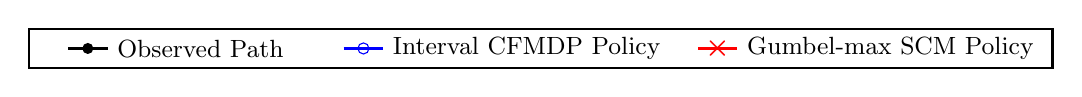
\begin{tikzpicture}[scale=1.0, every node/.style={scale=1.0}]
            \draw[thick, black] (-3, -0.25) rectangle (10, 0.25);
            %
            \draw[black, line width=1pt] (-2.5, 0.0) -- (-2,0.0);
            \fill[black] (-2.25,0.0) circle (2pt); %
            \node[right] at (-2,0.0) {\small Observed Path};
            
            %
            \draw[blue, line width=1pt] (1.0,0.0) -- (1.5,0.0);
            \node[draw=blue, circle, minimum size=4pt, inner sep=0pt] at (1.25,0.0) {}; %
            \node[right] at (1.5,0.0) {\small Interval CFMDP Policy};
            
            %
            \draw[red, line width=1pt] (5.5,0) -- (6,0);
            \node[red] at (5.75,0) {$\boldsymbol{\times}$}; %
            \node[right] at (6,0) {\small Gumbel-max SCM Policy};
        \end{tikzpicture}
    }\\
    %
    \subfigure[\footnotesize Lowest cumulative reward: Interval CFMDP ($312$), Gumbel-max SCM ($312$)]{%
        \resizebox{0.76\columnwidth}{!}{
             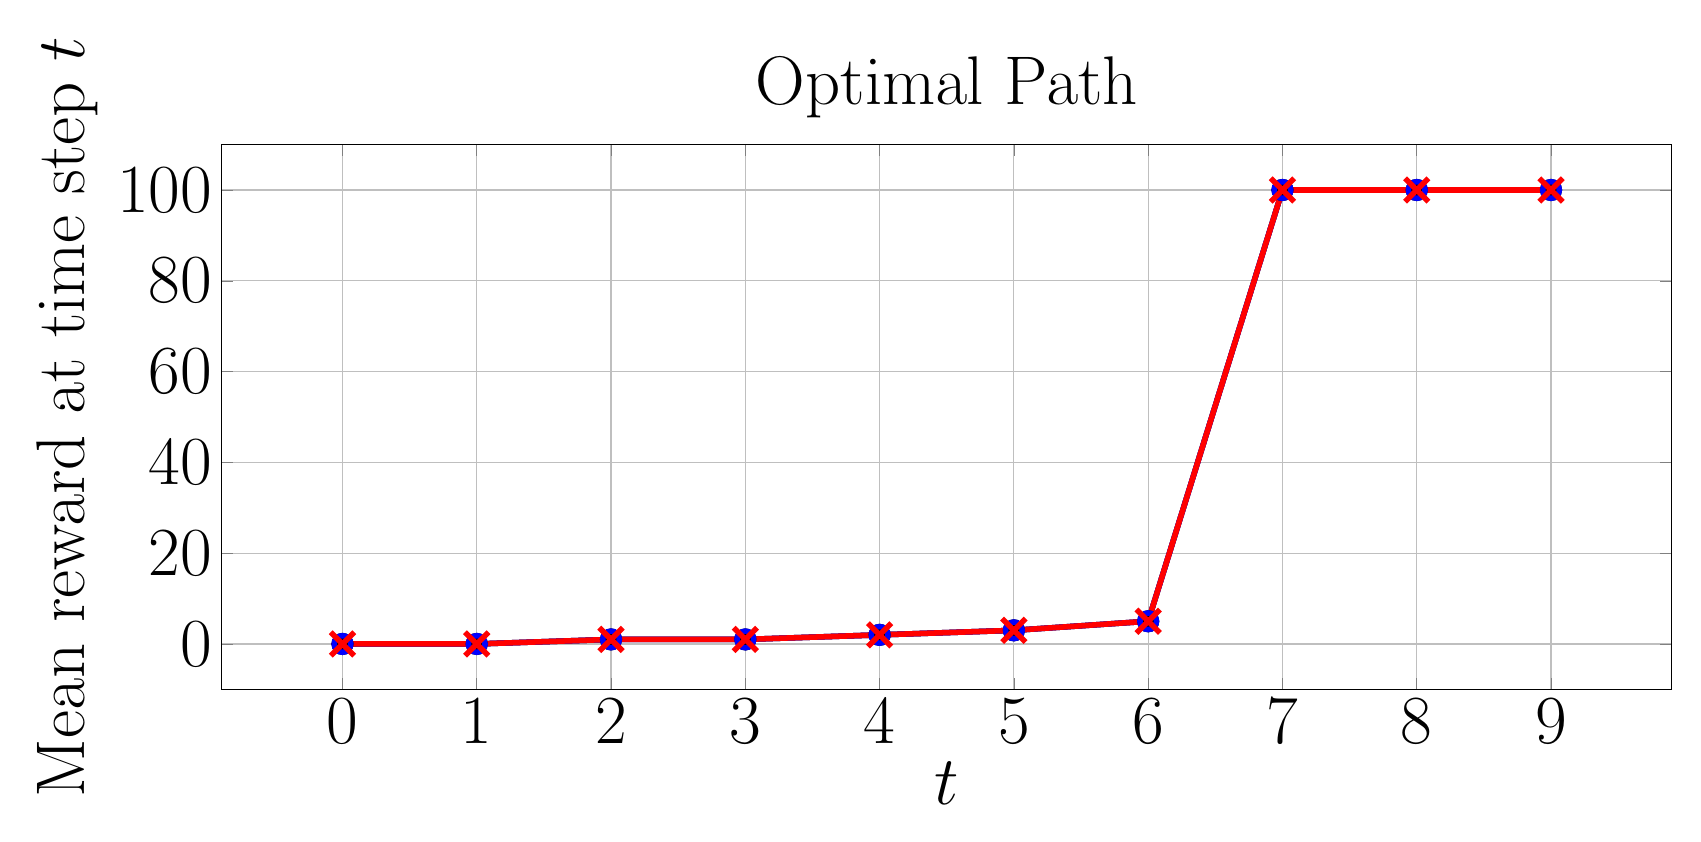
\begin{tikzpicture}
                \begin{axis}[
                    xlabel={$t$},
                    ylabel={Mean reward at time step $t$},
                    title={Optimal Path},
                    grid=both,
                    width=20cm, height=8.5cm,
                    every axis/.style={font=\Huge},
                    %
                ]
                \addplot[
                    color=black, %
                    mark=*, %
                    line width=2pt,
                    mark size=3pt,
                    error bars/.cd,
                    y dir=both, %
                    y explicit, %
                    error bar style={line width=1pt,solid},
                    error mark options={line width=1pt,mark size=4pt,rotate=90}
                ]
                coordinates {
                    (0, 0.0)  +- (0, 0.0)
                    (1, 0.0)  +- (0, 0.0) 
                    (2, 1.0)  +- (0, 0.0) 
                    (3, 1.0)  +- (0, 0.0)
                    (4, 2.0)  +- (0, 0.0)
                    (5, 3.0) +- (0, 0.0)
                    (6, 5.0) +- (0, 0.0)
                    (7, 100.0) +- (0, 0.0)
                    (8, 100.0) +- (0, 0.0)
                    (9, 100.0) +- (0, 0.0)
                };
                %
                \addplot[
                    color=blue, %
                    mark=o, %
                    line width=2pt,
                    mark size=3pt,
                    error bars/.cd,
                    y dir=both, %
                    y explicit, %
                    error bar style={line width=1pt,solid},
                    error mark options={line width=1pt,mark size=4pt,rotate=90}
                ]
                 coordinates {
                    (0, 0.0)  +- (0, 0.0)
                    (1, 0.0)  +- (0, 0.0) 
                    (2, 1.0)  +- (0, 0.0) 
                    (3, 1.0)  +- (0, 0.0)
                    (4, 2.0)  +- (0, 0.0)
                    (5, 3.0) +- (0, 0.0)
                    (6, 5.0) +- (0, 0.0)
                    (7, 100.0) +- (0, 0.0)
                    (8, 100.0) +- (0, 0.0)
                    (9, 100.0) +- (0, 0.0)
                };
                %
                \addplot[
                    color=red, %
                    mark=x, %
                    line width=2pt,
                    mark size=6pt,
                    error bars/.cd,
                    y dir=both, %
                    y explicit, %
                    error bar style={line width=1pt,solid},
                    error mark options={line width=1pt,mark size=4pt,rotate=90}
                ]
                coordinates {
                    (0, 0.0)  +- (0, 0.0)
                    (1, 0.0)  +- (0, 0.0) 
                    (2, 1.0)  +- (0, 0.0) 
                    (3, 1.0)  +- (0, 0.0)
                    (4, 2.0)  +- (0, 0.0)
                    (5, 3.0) +- (0, 0.0)
                    (6, 5.0) +- (0, 0.0)
                    (7, 100.0) +- (0, 0.0)
                    (8, 100.0) +- (0, 0.0)
                    (9, 100.0) +- (0, 0.0)
                };
                \end{axis}
            \end{tikzpicture}
         }
    }
    \hspace{1cm}
    \subfigure[\footnotesize Lowest cumulative reward: Interval CFMDP ($19$), Gumbel-max SCM ($-88$)]{%
         \resizebox{0.76\columnwidth}{!}{
            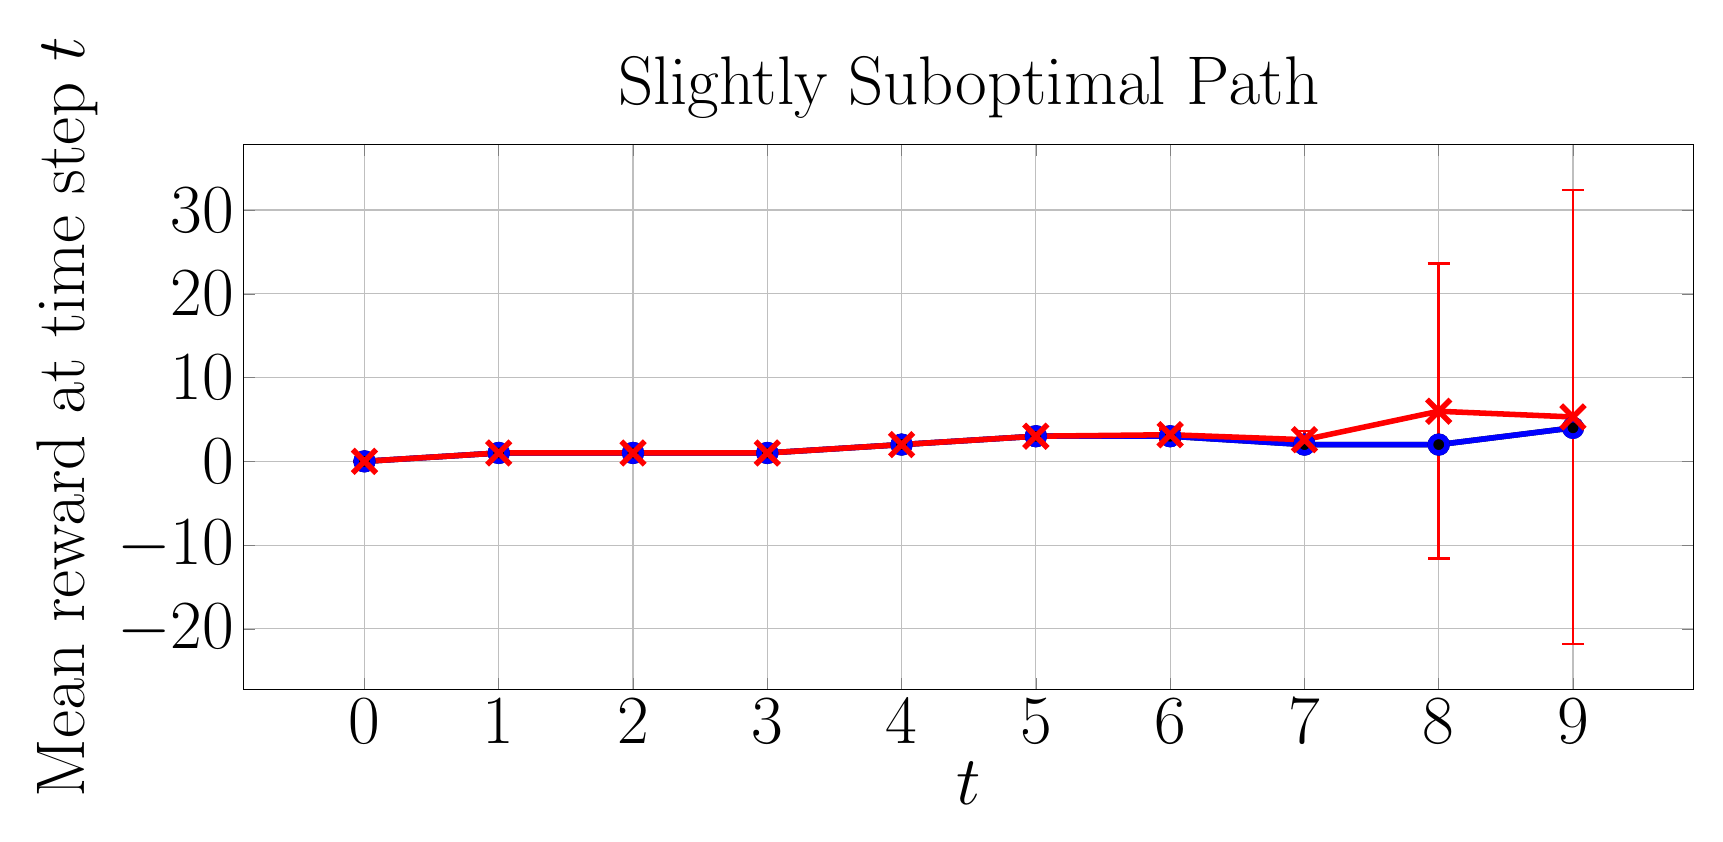
\begin{tikzpicture}
                \begin{axis}[
                    xlabel={$t$},
                    ylabel={Mean reward at time step $t$},
                    title={Slightly Suboptimal Path},
                    grid=both,
                    width=20cm, height=8.5cm,
                    every axis/.style={font=\Huge},
                    %
                ]
                \addplot[
                    color=black, %
                    mark=*, %
                    line width=2pt,
                    mark size=3pt,
                    error bars/.cd,
                    y dir=both, %
                    y explicit, %
                    error bar style={line width=1pt,solid},
                    error mark options={line width=1pt,mark size=4pt,rotate=90}
                ]
              coordinates {
                    (0, 0.0)  +- (0, 0.0)
                    (1, 1.0)  +- (0, 0.0) 
                    (2, 1.0)  +- (0, 0.0) 
                    (3, 1.0)  +- (0, 0.0)
                    (4, 2.0)  +- (0, 0.0)
                    (5, 3.0) +- (0, 0.0)
                    (6, 3.0) +- (0, 0.0)
                    (7, 2.0) +- (0, 0.0)
                    (8, 2.0) +- (0, 0.0)
                    (9, 4.0) +- (0, 0.0)
                };
                %
                \addplot[
                    color=blue, %
                    mark=o, %
                    line width=2pt,
                    mark size=3pt,
                    error bars/.cd,
                    y dir=both, %
                    y explicit, %
                    error bar style={line width=1pt,solid},
                    error mark options={line width=1pt,mark size=4pt,rotate=90}
                ]
              coordinates {
                    (0, 0.0)  +- (0, 0.0)
                    (1, 1.0)  +- (0, 0.0) 
                    (2, 1.0)  +- (0, 0.0) 
                    (3, 1.0)  +- (0, 0.0)
                    (4, 2.0)  +- (0, 0.0)
                    (5, 3.0) +- (0, 0.0)
                    (6, 3.0) +- (0, 0.0)
                    (7, 2.0) +- (0, 0.0)
                    (8, 2.0) +- (0, 0.0)
                    (9, 4.0) +- (0, 0.0)
                };
                %
                \addplot[
                    color=red, %
                    mark=x, %
                    line width=2pt,
                    mark size=6pt,
                    error bars/.cd,
                    y dir=both, %
                    y explicit, %
                    error bar style={line width=1pt,solid},
                    error mark options={line width=1pt,mark size=4pt,rotate=90}
                ]
                coordinates {
                    (0, 0.0)  +- (0, 0.0)
                    (1, 1.0)  +- (0, 0.0) 
                    (2, 1.0)  +- (0, 0.0) 
                    (3, 1.0)  +- (0, 0.0)
                    (4, 2.0)  += (0, 0.0)
                    (5, 3.0)  += (0, 0.0)
                    (6, 3.17847) += (0, 0.62606746) -= (0, 0.62606746)
                    (7, 2.5832885) += (0, 1.04598233) -= (0, 1.04598233)
                    (8, 5.978909) += (0, 17.60137623) -= (0, 17.60137623)
                    (9, 5.297059) += (0, 27.09227512) -= (0, 27.09227512)
                };
                \end{axis}
            \end{tikzpicture}
         }
    }\\[-1.5pt]
    \subfigure[\footnotesize Lowest cumulative reward: Interval CFMDP ($14$), Gumbel-max SCM ($-598$)]{%
         \resizebox{0.76\columnwidth}{!}{
             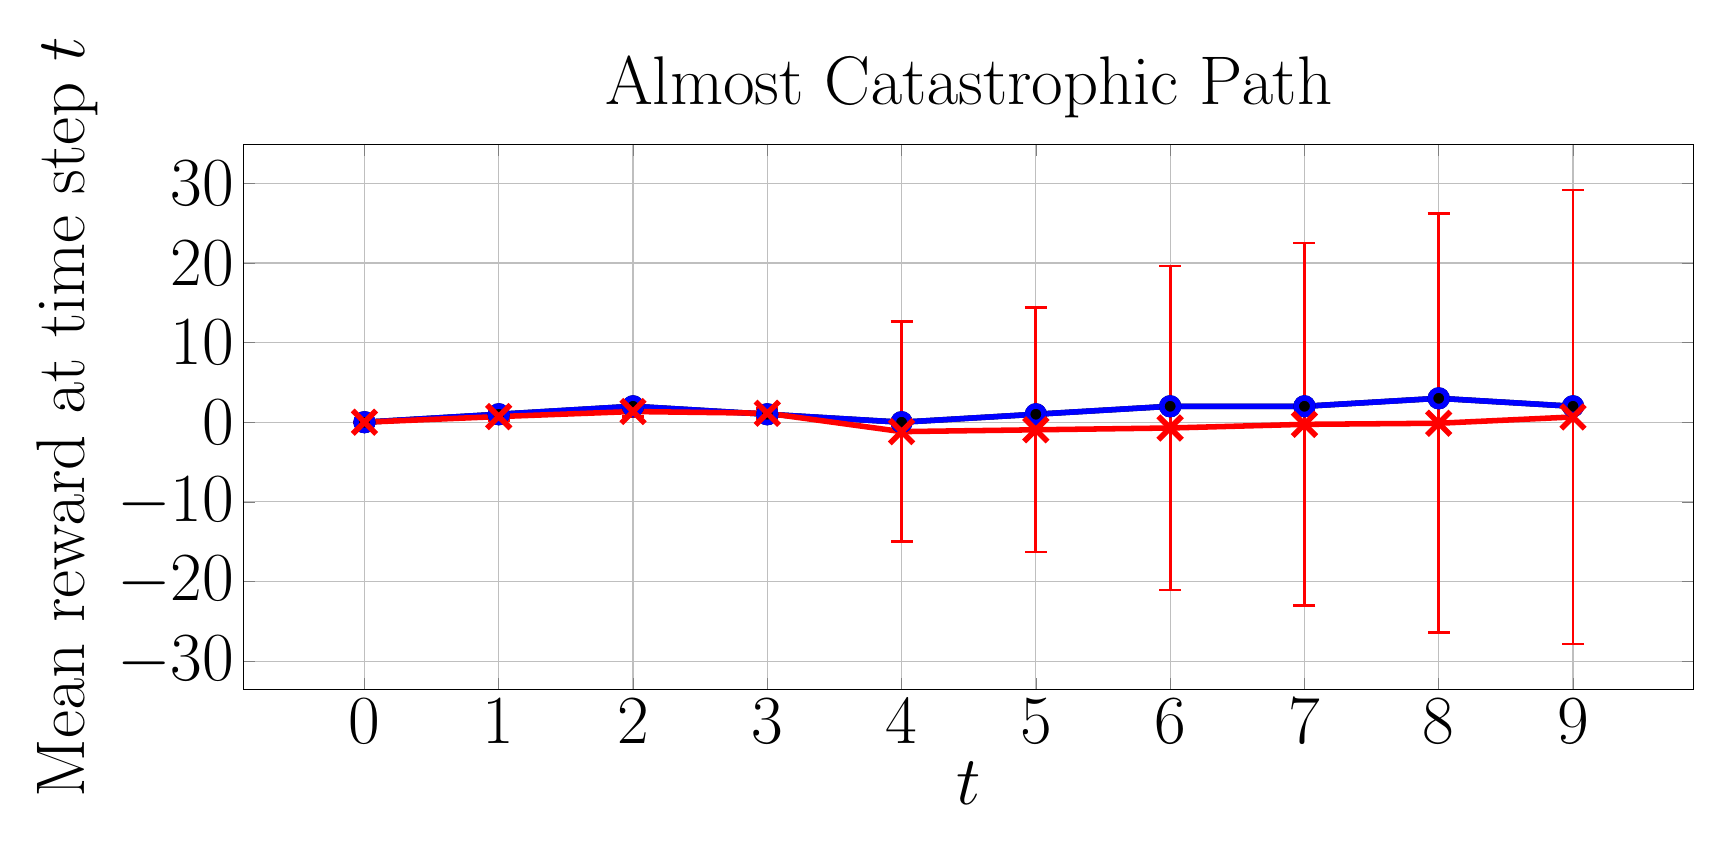
\begin{tikzpicture}
                \begin{axis}[
                    xlabel={$t$},
                    ylabel={Mean reward at time step $t$},
                    title={Almost Catastrophic Path},
                    grid=both,
                    width=20cm, height=8.5cm,
                    every axis/.style={font=\Huge},
                    %
                ]
                \addplot[
                    color=black, %
                    mark=*, %
                    line width=2pt,
                    mark size=3pt,
                    error bars/.cd,
                    y dir=both, %
                    y explicit, %
                    error bar style={line width=1pt,solid},
                    error mark options={line width=1pt,mark size=4pt,rotate=90}
                ]
                coordinates {
                    (0, 0.0)  +- (0, 0.0)
                    (1, 1.0)  +- (0, 0.0) 
                    (2, 2.0)  +- (0, 0.0) 
                    (3, 1.0)  +- (0, 0.0)
                    (4, 0.0)  +- (0, 0.0)
                    (5, 1.0) +- (0, 0.0)
                    (6, 2.0) +- (0, 0.0)
                    (7, 2.0) +- (0, 0.0)
                    (8, 3.0) +- (0, 0.0)
                    (9, 2.0) +- (0, 0.0)
                };
                %
                \addplot[
                    color=blue, %
                    mark=o, %
                    line width=2pt,
                    mark size=3pt,
                    error bars/.cd,
                    y dir=both, %
                    y explicit, %
                    error bar style={line width=1pt,solid},
                    error mark options={line width=1pt,mark size=4pt,rotate=90}
                ]
                coordinates {
                    (0, 0.0)  +- (0, 0.0)
                    (1, 1.0)  +- (0, 0.0) 
                    (2, 2.0)  +- (0, 0.0) 
                    (3, 1.0)  +- (0, 0.0)
                    (4, 0.0)  +- (0, 0.0)
                    (5, 1.0) +- (0, 0.0)
                    (6, 2.0) +- (0, 0.0)
                    (7, 2.0) +- (0, 0.0)
                    (8, 3.0) +- (0, 0.0)
                    (9, 2.0) +- (0, 0.0)
                };
                %
                \addplot[
                    color=red, %
                    mark=x, %
                    line width=2pt,
                    mark size=6pt,
                    error bars/.cd,
                    y dir=both, %
                    y explicit, %
                    error bar style={line width=1pt,solid},
                    error mark options={line width=1pt,mark size=4pt,rotate=90}
                ]
                coordinates {
                    (0, 0.0)  +- (0, 0.0)
                    (1, 0.7065655)  +- (0, 0.4553358) 
                    (2, 1.341673)  +- (0, 0.67091621) 
                    (3, 1.122926)  +- (0, 0.61281824)
                    (4, -1.1821935)  +- (0, 13.82444042)
                    (5, -0.952399)  +- (0, 15.35195457)
                    (6, -0.72672) +- (0, 20.33508414)
                    (7, -0.268983) +- (0, 22.77861454)
                    (8, -0.1310835) +- (0, 26.31013314)
                    (9, 0.65806) +- (0, 28.50670214)
                };
                %
            %
            %
            %
            %
            %
            %
            %
            %
            %
            %
            %
            %
            %
            %
            %
            %
            %
            %
                \end{axis}
            \end{tikzpicture}
         }
    }
    \hspace{1cm}
    \subfigure[\footnotesize Lowest cumulative reward: Interval CFMDP ($-698$), Gumbel-max SCM ($-698$)]{%
         \resizebox{0.76\columnwidth}{!}{
            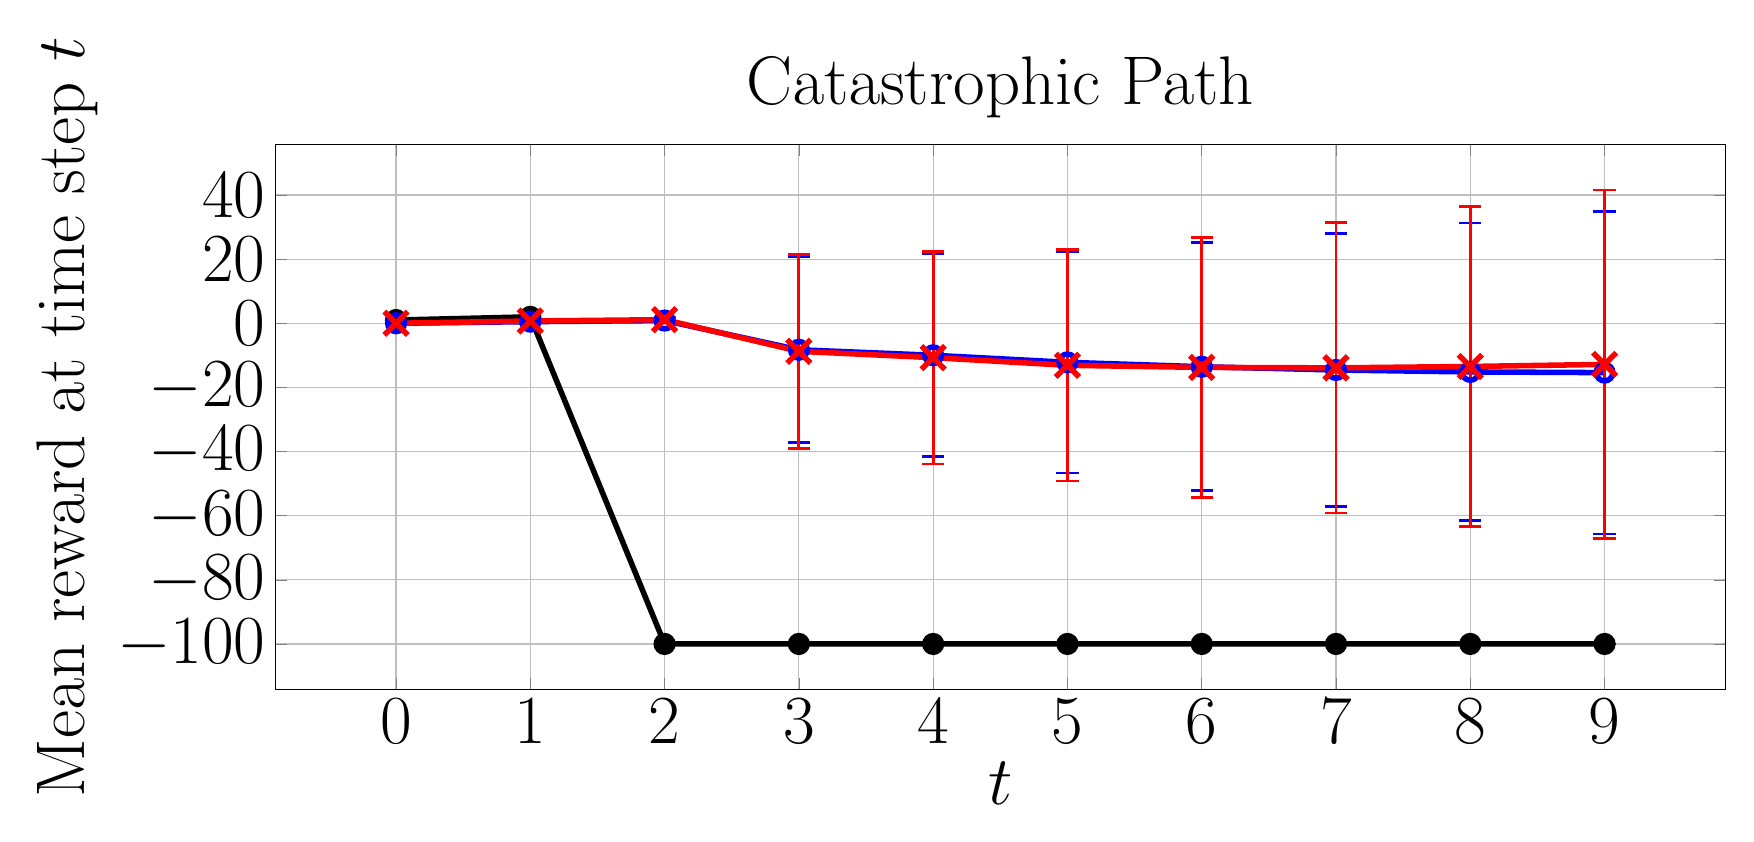
\begin{tikzpicture}
                \begin{axis}[
                    xlabel={$t$},
                    ylabel={Mean reward at time step $t$},
                    title={Catastrophic Path},
                    grid=both,
                    width=20cm, height=8.5cm,
                    every axis/.style={font=\Huge},
                    %
                ]
                \addplot[
                    color=black, %
                    mark=*, %
                    line width=2pt,
                    mark size=3pt,
                    error bars/.cd,
                    y dir=both, %
                    y explicit, %
                    error bar style={line width=1pt,solid},
                    error mark options={line width=1pt,mark size=4pt,rotate=90}
                ]
                coordinates {
                    (0, 1.0)  +- (0, 0.0)
                    (1, 2.0)  +- (0, 0.0) 
                    (2, -100.0)  +- (0, 0.0) 
                    (3, -100.0)  +- (0, 0.0)
                    (4, -100.0)  +- (0, 0.0)
                    (5, -100.0) +- (0, 0.0)
                    (6, -100.0) +- (0, 0.0)
                    (7, -100.0) +- (0, 0.0)
                    (8, -100.0) +- (0, 0.0)
                    (9, -100.0) +- (0, 0.0)
                };
                %
                \addplot[
                    color=blue, %
                    mark=o, %
                    line width=2pt,
                    mark size=3pt,
                    error bars/.cd,
                    y dir=both, %
                    y explicit, %
                    error bar style={line width=1pt,solid},
                    error mark options={line width=1pt,mark size=4pt,rotate=90}
                ]
                coordinates {
                    (0, 0.0)  +- (0, 0.0)
                    (1, 0.504814)  +- (0, 0.49997682) 
                    (2, 0.8439835)  +- (0, 0.76831917) 
                    (3, -8.2709165)  +- (0, 28.93656754)
                    (4, -9.981082)  +- (0, 31.66825363)
                    (5, -12.1776325) +- (0, 34.53463233)
                    (6, -13.556076) +- (0, 38.62845372)
                    (7, -14.574418) +- (0, 42.49603359)
                    (8, -15.1757075) +- (0, 46.41913968)
                    (9, -15.3900395) +- (0, 50.33563368)
                };
                %
                \addplot[
                    color=red, %
                    mark=x, %
                    line width=2pt,
                    mark size=6pt,
                    error bars/.cd,
                    y dir=both, %
                    y explicit, %
                    error bar style={line width=1pt,solid},
                    error mark options={line width=1pt,mark size=4pt,rotate=90}
                ]
                coordinates {
                    (0, 0.0)  +- (0, 0.0)
                    (1, 0.701873)  +- (0, 0.45743556) 
                    (2, 1.1227805)  +- (0, 0.73433129) 
                    (3, -8.7503255)  +- (0, 30.30257976)
                    (4, -10.722092)  +- (0, 33.17618589)
                    (5, -13.10721)  +- (0, 36.0648089)
                    (6, -13.7631645) +- (0, 40.56553451)
                    (7, -13.909043) +- (0, 45.23829402)
                    (8, -13.472517) +- (0, 49.96270296)
                    (9, -12.8278835) +- (0, 54.38618735)
                };
                %
            %
            %
            %
            %
            %
            %
            %
            %
            %
            %
            %
            %
            %
            %
            %
            %
            %
            %
                \end{axis}
            \end{tikzpicture}
         }
    }
    \caption{Average instant reward of CF paths induced by policies on GridWorld $p=0.4$.}
    \label{fig: reward p=0.4}
\end{figure*}

\subsection{Experimental Setup}
To compare policy performance, we measure the average rewards of counterfactual paths induced by our policy and the Gumbel-max policy by uniformly sampling $200$ counterfactual MDPs from the ICFMDP and generating $10,000$ counterfactual paths over each sampled CFMDP. \jl{Since the interval CFMDP depends on the observed path, we select $4$  paths of varying optimality to evaluate how the observed path impacts the performance of both policies: an optimal path, a slightly suboptimal path that could reach the optimal reward with a few changes, a catastrophic path that enters a catastrophic, terminal state with low reward, and an almost catastrophic path that was close to entering a catastrophic state.} When measuring the average probability bound widths and execution time needed to generate the ICFMDPs, we averaged over $20$ randomly generated observed paths
\footnote{Further training details are provided in Appendix \ref{app: training details}, and the code is provided at \href{https://github.com/ddv-lab/robust-cf-inference-in-MDPs}{https://github.com/ddv-lab/robust-cf-inference-in-MDPs}
%
%
.}.

\subsection{GridWorld}
\jl{The GridWorld MDP is a $4 \times 4$ grid where an agent must navigate from the top-left corner to the goal state in the bottom-right corner, avoiding a dangerous terminal state in the centre. At each time step, the agent can move up, down, left, or right, but there is a small probability (controlled by hyper-parameter $p$) of moving in an unintended direction. As the agent nears the goal, the reward for each state increases, culminating in a reward of $+100$ for reaching the goal. Entering the dangerous state results in a penalty of $-100$. We use two versions of GridWorld: a less stochastic version with $p=0.9$ (i.e., $90$\% chance of moving in the chosen direction) and a more stochastic version with $p=0.4$.}

\paragraph{GridWorld ($p=0.9$)}
When $p=0.9$, the counterfactual probability bounds are typically narrow (see Table \ref{tab:nonzero_probs} for average measurements). Consequently, as shown in Figure \ref{fig: reward p=0.9}, both policies are nearly identical and perform similarly well across the optimal, slightly suboptimal, and catastrophic paths.
%
However, for the almost catastrophic path, the interval CFMDP path is more conservative and follows the observed path more closely (as this is where the probability bounds are narrowest), which typically requires one additional step to reach the goal state than the Gumbel-max SCM policy.
%

\paragraph{GridWorld ($p=0.4$)}
\jl{When $p=0.4$, the GridWorld environment becomes more uncertain, increasing the risk of entering the dangerous state even if correct actions are chosen. Thus, as shown in Figure \ref{fig: reward p=0.4}, the interval CFMDP policy adopts a more conservative approach, avoiding deviation from the observed policy if it cannot guarantee higher counterfactual rewards (see the slightly suboptimal and almost catastrophic paths), whereas the Gumbel-max SCM is inconsistent: it can yield higher rewards, but also much lower rewards, reflected in the wide error bars.} For the catastrophic path, both policies must deviate from the observed path to achieve a higher reward and, in this case, perform similarly.
%
%
%
%
\subsection{Sepsis}
The Sepsis MDP \citep{oberst2019counterfactual} simulates trajectories of Sepsis patients. Each state consists of four vital signs (heart rate, blood pressure, oxygen concentration, and glucose levels), categorised as low, normal, or high.
and three treatments that can be toggled on/off at each time step (8 actions in total). Unlike \citet{oberst2019counterfactual}, we scale rewards based on the number of out-of-range vital signs, between $-1000$ (patient dies) and $1000$ (patient discharged). \jl{Like the GridWorld $p=0.4$ experiment, the Sepsis MDP is highly uncertain, as many states are equally likely to lead to optimal and poor outcomes. Thus, as shown in Figure \ref{fig: reward sepsis}, both policies follow the observed optimal and almost catastrophic paths to guarantee rewards are no worse than the observation.} However, improving the catastrophic path requires deviating from the observation. Here, the Gumbel-max SCM policy, on average, performs better than the interval CFMDP policy. But, since both policies have lower bounds clipped at $-1000$, neither policy reliably improves over the observation. In contrast, for the slightly suboptimal path, the interval CFMDP policy performs significantly better, shown by its higher lower bounds. 
Moreover, in these two cases, the worst-case counterfactual path generated by the interval CFMDP policy is better than that of the Gumbel-max SCM policy,
indicating its greater robustness.
%
\begin{figure*}
    \centering
     \resizebox{0.6\textwidth}{!}{
        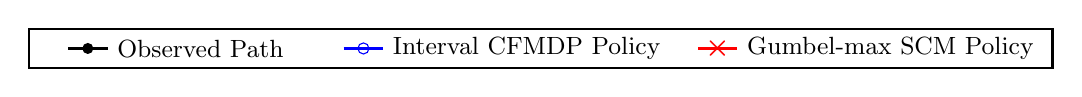
\begin{tikzpicture}[scale=1.0, every node/.style={scale=1.0}]
            \draw[thick, black] (-3, -0.25) rectangle (10, 0.25);
            %
            \draw[black, line width=1pt] (-2.5, 0.0) -- (-2,0.0);
            \fill[black] (-2.25,0.0) circle (2pt); %
            \node[right] at (-2,0.0) {\small Observed Path};
            
            %
            \draw[blue, line width=1pt] (1.0,0.0) -- (1.5,0.0);
            \node[draw=blue, circle, minimum size=4pt, inner sep=0pt] at (1.25,0.0) {}; %
            \node[right] at (1.5,0.0) {\small Interval CFMDP Policy};
            
            %
            \draw[red, line width=1pt] (5.5,0) -- (6,0);
            \node[red] at (5.75,0) {$\boldsymbol{\times}$}; %
            \node[right] at (6,0) {\small Gumbel-max SCM Policy};
        \end{tikzpicture}
    }\\
    \subfigure[\footnotesize Lowest cumulative reward: Interval CFMDP ($8000$), Gumbel-max SCM ($8000$)]{%
         \resizebox{0.76\columnwidth}{!}{
             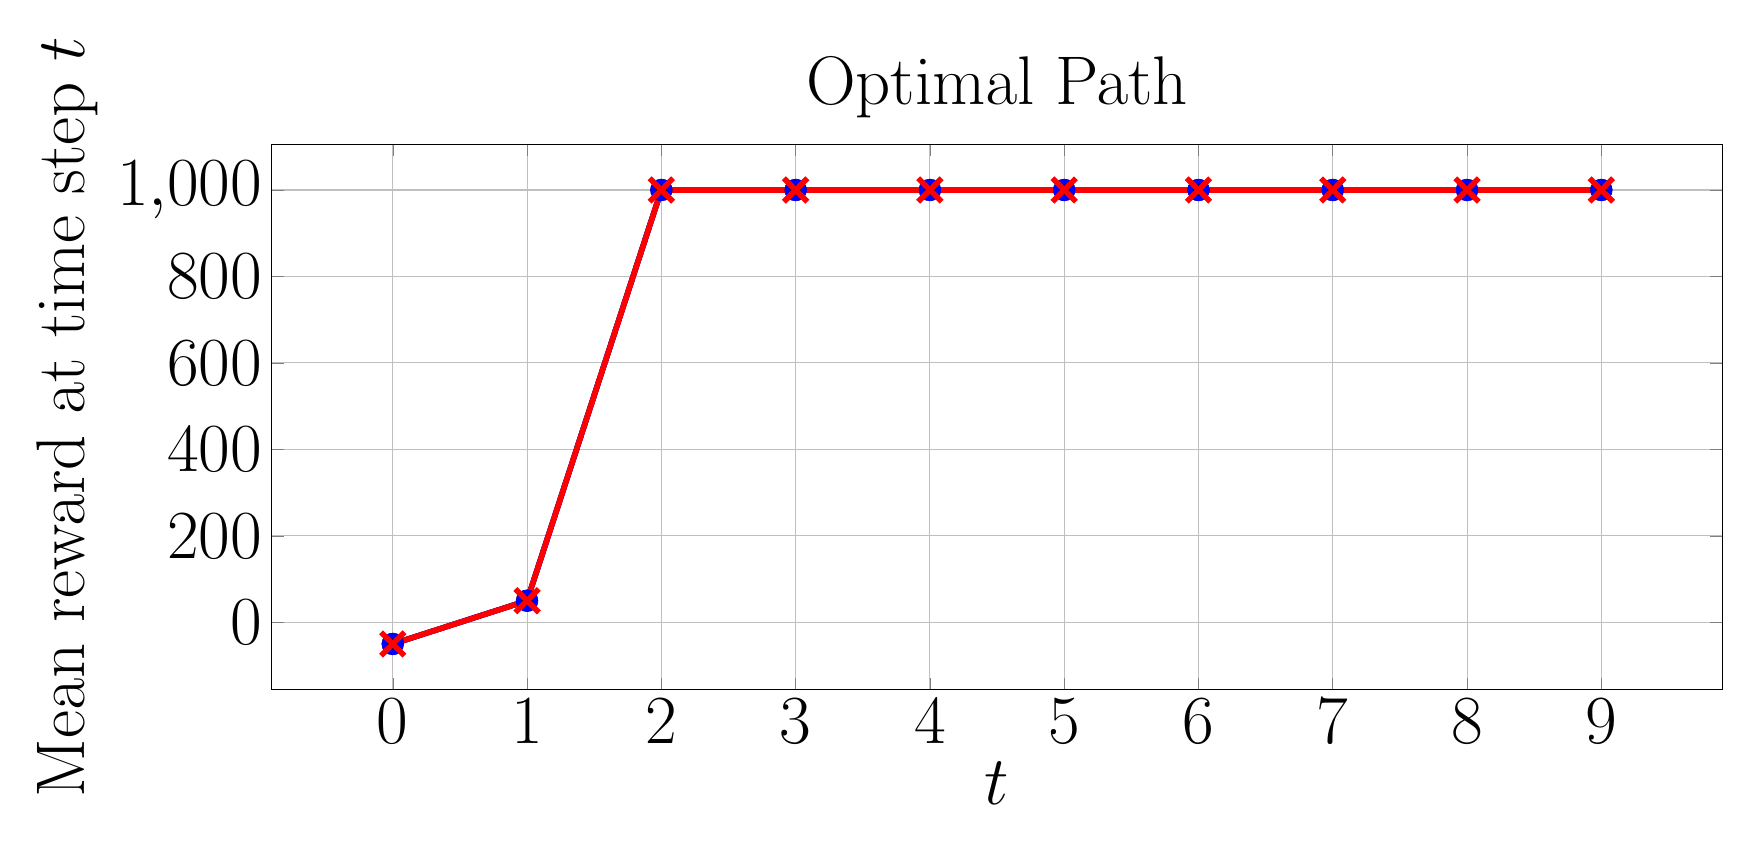
\begin{tikzpicture}
                \begin{axis}[
                    xlabel={$t$},
                    ylabel={Mean reward at time step $t$},
                    title={Optimal Path},
                    grid=both,
                    width=20cm, height=8.5cm,
                    every axis/.style={font=\Huge},
                    %
                ]
                \addplot[
                    color=black, %
                    mark=*, %
                    line width=2pt,
                    mark size=3pt,
                ]
                coordinates {
                    (0, -50.0)
                    (1, 50.0)
                    (2, 1000.0)
                    (3, 1000.0)
                    (4, 1000.0)
                    (5, 1000.0)
                    (6, 1000.0)
                    (7, 1000.0)
                    (8, 1000.0)
                    (9, 1000.0)
                };
                %
                \addplot[
                    color=blue, %
                    mark=o, %
                    line width=2pt,
                    mark size=3pt,
                    error bars/.cd,
                    y dir=both, %
                    y explicit, %
                    error bar style={line width=1pt,solid},
                    error mark options={line width=1pt,mark size=4pt,rotate=90}
                ]
                coordinates {
                    (0, -50.0)  +- (0, 0.0)
                    (1, 50.0)  +- (0, 0.0) 
                    (2, 1000.0)  +- (0, 0.0) 
                    (3, 1000.0)  +- (0, 0.0)
                    (4, 1000.0)  +- (0, 0.0)
                    (5, 1000.0) +- (0, 0.0)
                    (6, 1000.0) +- (0, 0.0)
                    (7, 1000.0) +- (0, 0.0)
                    (8, 1000.0) +- (0, 0.0)
                    (9, 1000.0) +- (0, 0.0)
                };
                %
                \addplot[
                    color=red, %
                    mark=x, %
                    line width=2pt,
                    mark size=6pt,
                    error bars/.cd,
                    y dir=both, %
                    y explicit, %
                    error bar style={line width=1pt,solid},
                    error mark options={line width=1pt,mark size=4pt,rotate=90}
                ]
                coordinates {
                    (0, -50.0)  +- (0, 0.0)
                    (1, 50.0)  +- (0, 0.0) 
                    (2, 1000.0)  +- (0, 0.0) 
                    (3, 1000.0)  +- (0, 0.0)
                    (4, 1000.0)  +- (0, 0.0)
                    (5, 1000.0) +- (0, 0.0)
                    (6, 1000.0) +- (0, 0.0)
                    (7, 1000.0) +- (0, 0.0)
                    (8, 1000.0) +- (0, 0.0)
                    (9, 1000.0) +- (0, 0.0)
                };
                %
                \end{axis}
            \end{tikzpicture}
         }
    }
    \hspace{1cm}
    \subfigure[\footnotesize Lowest cumulative reward: Interval CFMDP ($-5980$), Gumbel-max SCM ($-8000$)]{%
         \resizebox{0.76\columnwidth}{!}{
            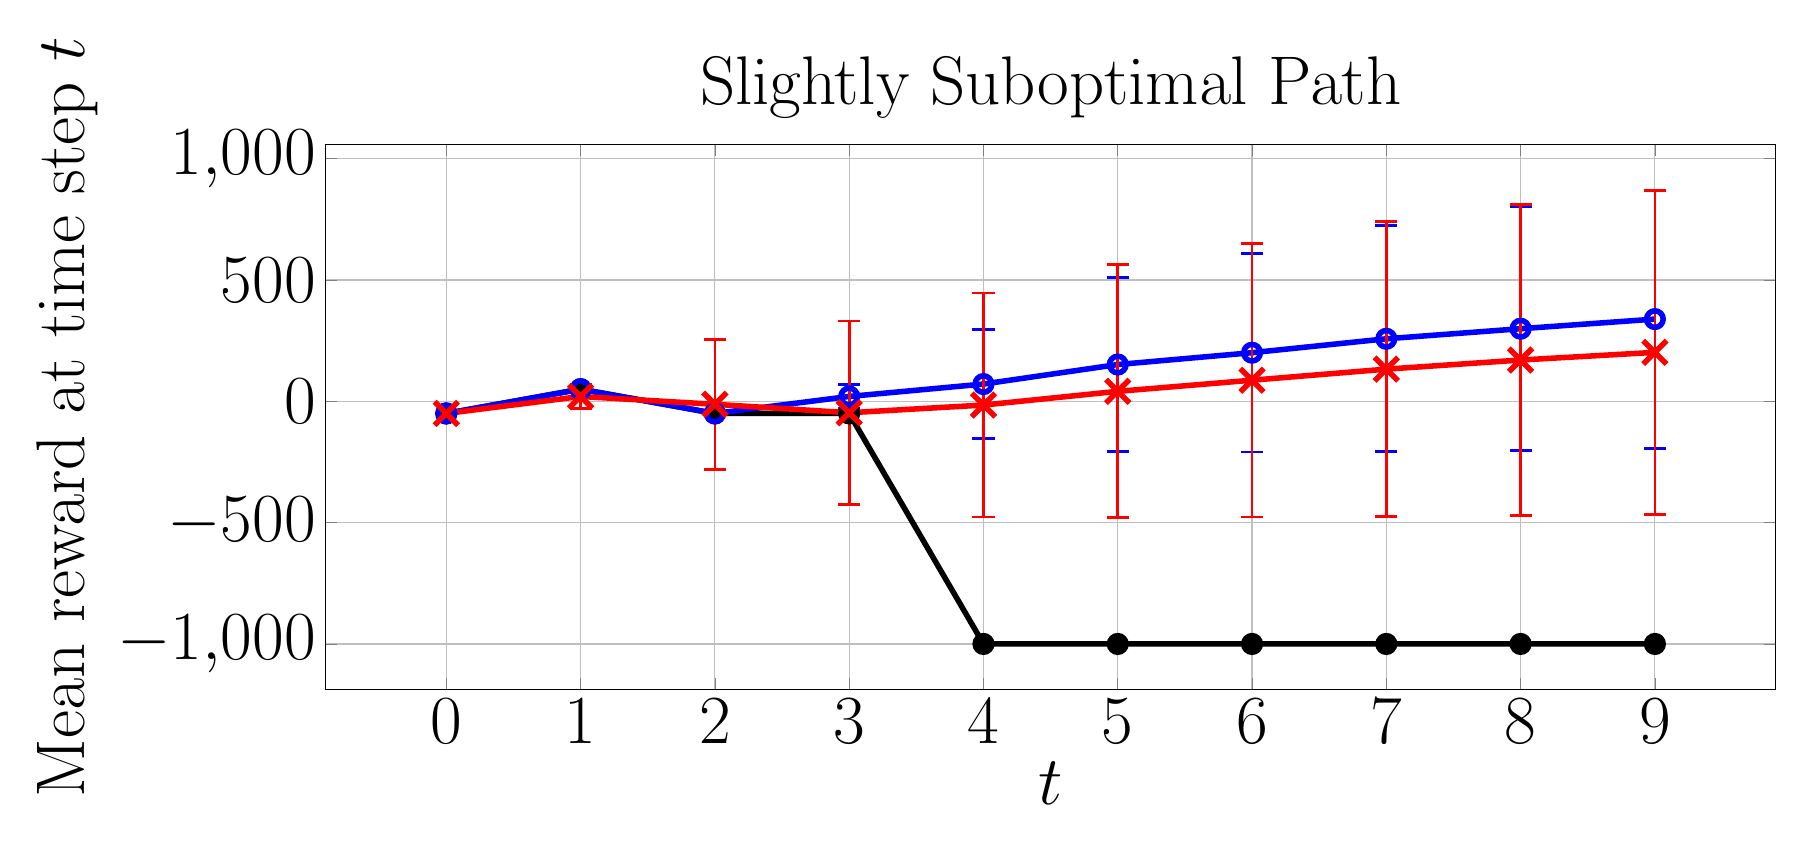
\begin{tikzpicture}
                \begin{axis}[
                    xlabel={$t$},
                    ylabel={Mean reward at time step $t$},
                    title={Slightly Suboptimal Path},
                    grid=both,
                    width=20cm, height=8.5cm,
                    every axis/.style={font=\Huge},
                    %
                ]
               \addplot[
                    color=black, %
                    mark=*, %
                    line width=2pt,
                    mark size=3pt,
                ]
                coordinates {
                    (0, -50.0)
                    (1, 50.0)
                    (2, -50.0)
                    (3, -50.0)
                    (4, -1000.0)
                    (5, -1000.0)
                    (6, -1000.0)
                    (7, -1000.0)
                    (8, -1000.0)
                    (9, -1000.0)
                };
                %
                \addplot[
                    color=blue, %
                    mark=o, %
                    line width=2pt,
                    mark size=3pt,
                    error bars/.cd,
                    y dir=both, %
                    y explicit, %
                    error bar style={line width=1pt,solid},
                    error mark options={line width=1pt,mark size=4pt,rotate=90}
                ]
                coordinates {
                    (0, -50.0)  +- (0, 0.0)
                    (1, 50.0)  +- (0, 0.0) 
                    (2, -50.0)  +- (0, 0.0) 
                    (3, 20.0631)  +- (0, 49.97539413)
                    (4, 71.206585)  +- (0, 226.02033693)
                    (5, 151.60797) +- (0, 359.23292559)
                    (6, 200.40593) +- (0, 408.86185176)
                    (7, 257.77948) +- (0, 466.10372804)
                    (8, 299.237465) +- (0, 501.82579506)
                    (9, 338.9129) +- (0, 532.06124996)
                };
                %
                \addplot[
                    color=red, %
                    mark=x, %
                    line width=2pt,
                    mark size=6pt,
                    error bars/.cd,
                    y dir=both, %
                    y explicit, %
                    error bar style={line width=1pt,solid},
                    error mark options={line width=1pt,mark size=4pt,rotate=90}
                ]
                coordinates {
                    (0, -50.0)  +- (0, 0.0)
                    (1, 20.00736)  +- (0, 49.99786741) 
                    (2, -12.282865)  +- (0, 267.598755) 
                    (3, -47.125995)  +- (0, 378.41755832)
                    (4, -15.381965)  +- (0, 461.77616558)
                    (5, 41.15459) +- (0, 521.53189262)
                    (6, 87.01595) +- (0, 564.22243126 )
                    (7, 132.62376) +- (0, 607.31338037)
                    (8, 170.168145) +- (0, 641.48013693)
                    (9, 201.813135) +- (0, 667.29441777)
                };
                %
                %
                %
                %
                %
                %
                %
                %
                %
                %
                %
                %
                %
                %
                %
                %
                %
                %
                %
                \end{axis}
            \end{tikzpicture}
         }
    }\\[-1.5pt]
    \subfigure[\footnotesize Lowest cumulative reward: Interval CFMDP ($100$), Gumbel-max SCM ($100$)]{%
         \resizebox{0.76\columnwidth}{!}{
             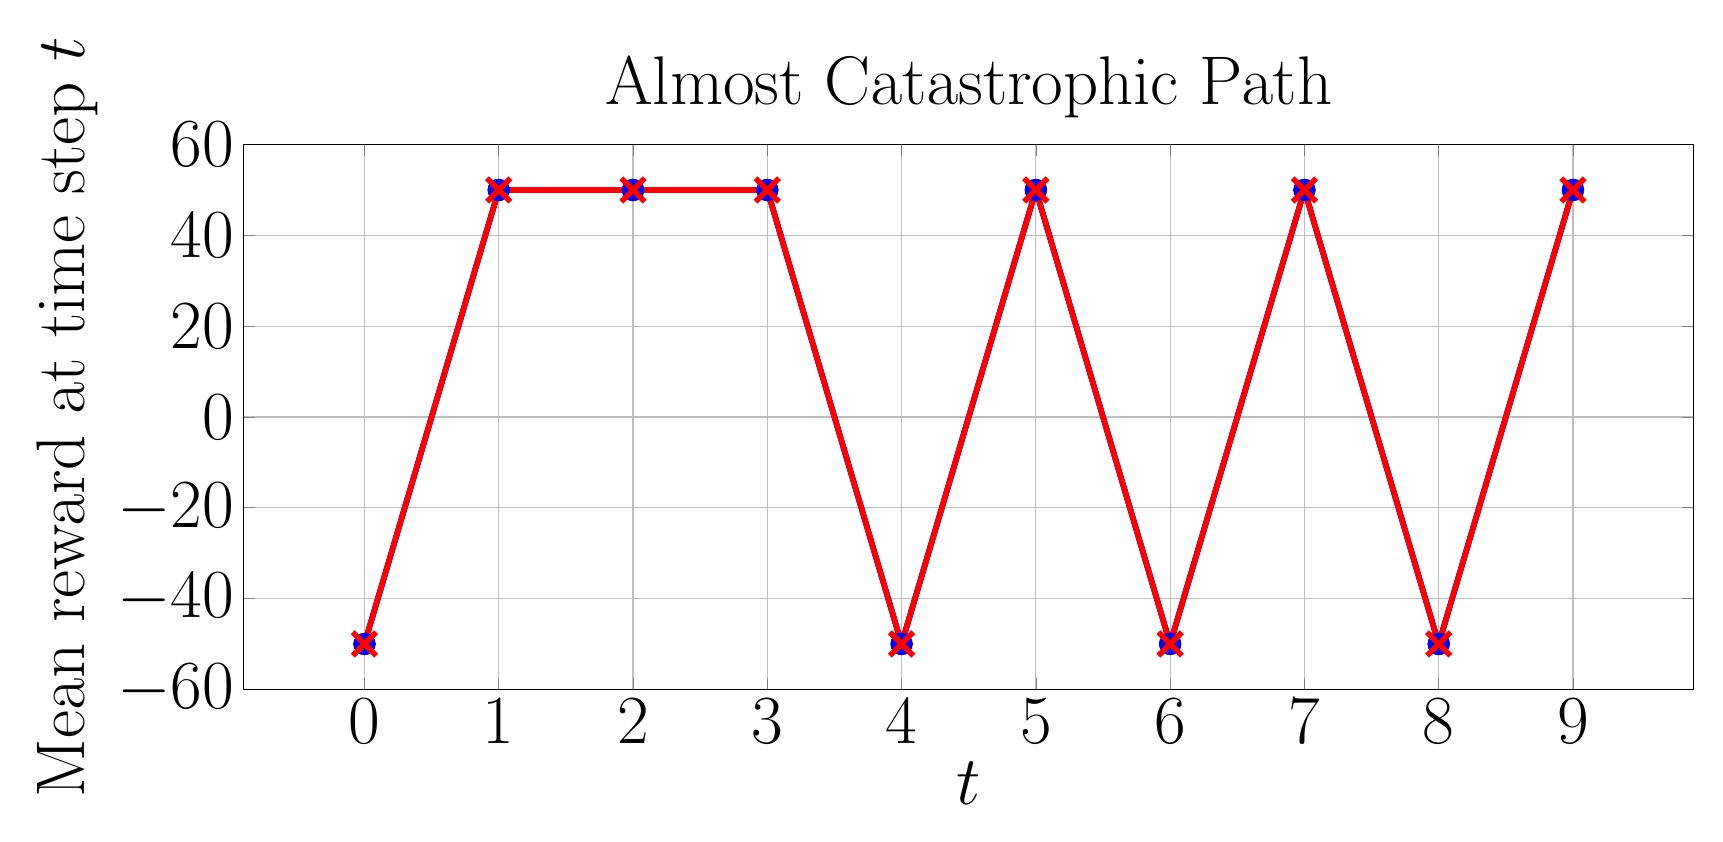
\begin{tikzpicture}
                \begin{axis}[
                    xlabel={$t$},
                    ylabel={Mean reward at time step $t$},
                    title={Almost Catastrophic Path},
                    grid=both,
                    every axis/.style={font=\Huge},
                    width=20cm, height=8.5cm,
                    %
                ]
               \addplot[
                    color=black, %
                    mark=*, %
                    line width=2pt,
                    mark size=3pt,
                ]
                coordinates {
                    (0, -50.0)
                    (1, 50.0)
                    (2, 50.0)
                    (3, 50.0)
                    (4, -50.0)
                    (5, 50.0)
                    (6, -50.0)
                    (7, 50.0)
                    (8, -50.0)
                    (9, 50.0)
                };
                %
                %
                \addplot[
                    color=blue, %
                    mark=o, %
                    line width=2pt,
                    mark size=3pt,
                    error bars/.cd,
                    y dir=both, %
                    y explicit, %
                    error bar style={line width=1pt,solid},
                    error mark options={line width=1pt,mark size=4pt,rotate=90}
                ]
                coordinates {
                    (0, -50.0)  +- (0, 0.0)
                    (1, 50.0)  +- (0, 0.0) 
                    (2, 50.0)  +- (0, 0.0) 
                    (3, 50.0)  +- (0, 0.0)
                    (4, -50.0)  +- (0, 0.0)
                    (5, 50.0) +- (0, 0.0)
                    (6, -50.0) +- (0, 0.0)
                    (7, 50.0) +- (0, 0.0)
                    (8, -50.0) +- (0, 0.0)
                    (9, 50.0) +- (0, 0.0)
                };
                %
                \addplot[
                    color=red, %
                    mark=x, %
                    line width=2pt,
                    mark size=6pt,
                    error bars/.cd,
                    y dir=both, %
                    y explicit, %
                    error bar style={line width=1pt,solid},
                    error mark options={line width=1pt,mark size=4pt,rotate=90}
                ]
                coordinates {
                    (0, -50.0)  +- (0, 0.0)
                    (1, 50.0)  +- (0, 0.0) 
                    (2, 50.0)  +- (0, 0.0) 
                    (3, 50.0)  +- (0, 0.0)
                    (4, -50.0)  +- (0, 0.0)
                    (5, 50.0) +- (0, 0.0)
                    (6, -50.0) +- (0, 0.0)
                    (7, 50.0) +- (0, 0.0)
                    (8, -50.0) +- (0, 0.0)
                    (9, 50.0) +- (0, 0.0)
                };
                %
                %
                %
                %
                %
                %
                %
                %
                %
                %
                %
                %
                %
                %
                %
                %
                %
                %
                %
                \end{axis}
            \end{tikzpicture}
         }
    }
    \hspace{1cm}
    \subfigure[\footnotesize Lowest cumulative reward: Interval CFMDP ($-7150$), Gumbel-max SCM ($-9050$)]{%
         \resizebox{0.76\columnwidth}{!}{
            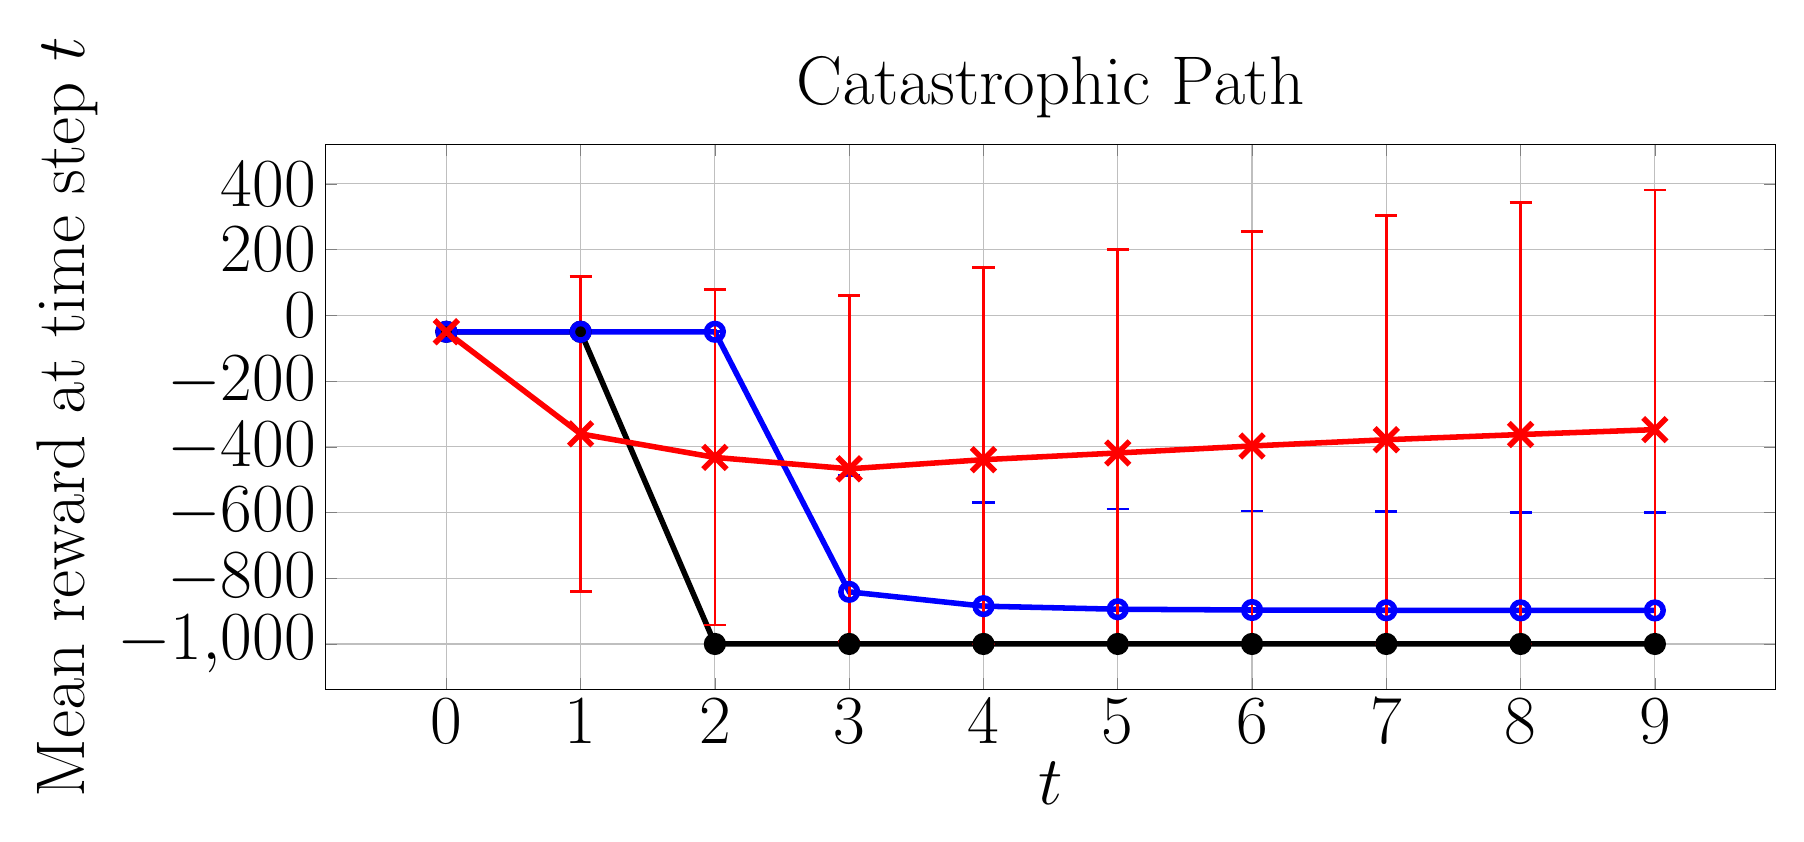
\begin{tikzpicture}
                \begin{axis}[
                    xlabel={$t$},
                    ylabel={Mean reward at time step $t$},
                    title={Catastrophic Path},
                    grid=both,
                    width=20cm, height=8.5cm,
                    every axis/.style={font=\Huge},
                    %
                ]
               \addplot[
                    color=black, %
                    mark=*, %
                    line width=2pt,
                    mark size=3pt,
                ]
                coordinates {
                    (0, -50.0)
                    (1, -50.0)
                    (2, -1000.0)
                    (3, -1000.0)
                    (4, -1000.0)
                    (5, -1000.0)
                    (6, -1000.0)
                    (7, -1000.0)
                    (8, -1000.0)
                    (9, -1000.0)
                };
                %
                %
                \addplot[
                    color=blue, %
                    mark=o, %
                    line width=2pt,
                    mark size=3pt,
                    error bars/.cd,
                    y dir=both, %
                    y explicit, %
                    error bar style={line width=1pt,solid},
                    error mark options={line width=1pt,mark size=4pt,rotate=90}
                ]
                coordinates {
                    (0, -50.0)  +- (0, 0.0)
                    (1, -50.0)  +- (0, 0.0) 
                    (2, -50.0)  +- (0, 0.0) 
                    (3, -841.440725)  += (0, 354.24605512) -= (0, 158.559275)
                    (4, -884.98225)  += (0, 315.37519669) -= (0, 115.01775)
                    (5, -894.330425) += (0, 304.88572805) -= (0, 105.669575)
                    (6, -896.696175) += (0, 301.19954514) -= (0, 103.303825)
                    (7, -897.4635) += (0, 299.61791279) -= (0, 102.5365)
                    (8, -897.77595) += (0, 298.80392585) -= (0, 102.22405)
                    (9, -897.942975) += (0, 298.32920557) -= (0, 102.057025)
                };
                %
                \addplot[
                    color=red, %
                    mark=x, %
                    line width=2pt,
                    mark size=6pt,
                    error bars/.cd,
                    y dir=both, %
                    y explicit, %
                    error bar style={line width=1pt,solid},
                    error mark options={line width=1pt,mark size=4pt,rotate=90}
                ]
            coordinates {
                    (0, -50.0)  +- (0, 0.0)
                    (1, -360.675265)  +- (0, 479.39812699) 
                    (2, -432.27629)  +- (0, 510.38620897) 
                    (3, -467.029545)  += (0, 526.36009628) -= (0, 526.36009628)
                    (4, -439.17429)  += (0, 583.96638919) -= (0, 560.82571)
                    (5, -418.82704) += (0, 618.43027478) -= (0, 581.17296)
                    (6, -397.464895) += (0, 652.67322574) -= (0, 602.535105)
                    (7, -378.49052) += (0, 682.85407033) -= (0, 621.50948)
                    (8, -362.654195) += (0, 707.01412023) -= (0, 637.345805)
                    (9, -347.737935) += (0, 729.29076479) -= (0, 652.262065)
                };
                %
                %
                %
                %
                %
                %
                %
                %
                %
                %
                %
                %
                %
                %
                %
                %
                %
                %
                %
                \end{axis}
            \end{tikzpicture}
         }
    }
    \caption{Average instant reward of CF paths induced by policies on Sepsis.}
    \label{fig: reward sepsis}
\end{figure*}

%
%
%
\subsection{Interval CFMDP Bounds}
%
%
Table \ref{tab:nonzero_probs} presents the mean counterfactual probability bound widths (excluding transitions where the upper bound is $0$) for each MDP, averaged over 20 observed paths. We compare the bounds under counterfactual stability (CS) and monotonicity (M) assumptions, CS alone, and no assumptions. This shows that the assumptions marginally reduce the bound widths, indicating the assumptions tighten the bounds without excluding too many causal models, as intended.
\renewcommand{\arraystretch}{1}

\begin{table}
\centering
\caption{Mean width of counterfactual probability bounds}
\resizebox{0.8\columnwidth}{!}{%
\begin{tabular}{|c|c|c|c|}
\hline
\multirow{2}{*}{\textbf{Environment}} & \multicolumn{3}{c|}{\textbf{Assumptions}} \\ \cline{2-4}
 & \textbf{CS + M} & \textbf{CS} & \textbf{None\tablefootnote{\jl{Equivalent to \citet{li2024probabilities}'s bounds (see Section \ref{sec: equivalence with Li}).}}} \\ \hline
\textbf{GridWorld} ($p=0.9$) & 0.0817 & 0.0977 & 0.100 \\ \hline
\textbf{GridWorld} ($p=0.4$) & 0.552  & 0.638  & 0.646 \\ \hline
\textbf{Sepsis} & 0.138 & 0.140 & 0.140 \\ \hline
\end{tabular}
}
\label{tab:nonzero_probs}
\end{table}


\subsection{Execution Times}
Table \ref{tab: times} compares the average time needed to generate the interval CFMDP vs.\ the Gumbel-max SCM CFMDP for 20 observations.
The GridWorld algorithms were run single-threaded, while the Sepsis experiments were run in parallel.
Generating the interval CFMDP is significantly faster as it uses exact analytical bounds, whereas the Gumbel-max CFMDP requires sampling from the Gumbel distribution to estimate counterfactual transition probabilities. \jl{Since constructing the counterfactual MDP models is the main bottleneck in both approaches, ours is more efficient overall and suitable for larger MDPs.}
\begin{table}
\centering
\caption{Mean execution time to generate CFMDPs}
\resizebox{0.99\columnwidth}{!}{%
\begin{tabular}{|c|c|c|}
\hline
\multirow{2}{*}{\textbf{Environment}} & \multicolumn{2}{c|}{\textbf{Mean Execution Time (s)}} \\ \cline{2-3} 
                                      & \textbf{Interval CFMDP} & \textbf{Gumbel-max CFMDP} \\ \hline
\textbf{GridWorld ($p=0.9$) }                  & 0.261                   & 56.1                      \\ \hline
\textbf{GridWorld ($p=0.4$)  }                 & 0.336                   & 54.5                      \\ \hline
\textbf{Sepsis}                                 & 688                     & 2940                      \\ \hline
\end{tabular}%
}
\label{tab: times}
\end{table}


% \begin{wraptable}{r}{0.65\textwidth}
% \centering
% \caption{The comparison of resource requirements between Eurus-2-7B-PRIME and Qwen2.5-Math-7B-Instruct.}
% \label{tab:comparision}
% \resizebox{0.65\textwidth}{!}{
% \begin{tabular}{l >{\columncolor[HTML]{D7E8E8}}l l}
% \toprule
% \textbf{Model} & \textbf{Eurus-2-7B-PRIME} & \textbf{Qwen2.5-Math-7B-Instruct} \\ \midrule
% Base Model     & Qwen2.5-Math-7B           & Qwen2.5-Math-7B                  \\
% SFT Data       & 230K (open-source)        & 2.5M (open-source and in-house)  \\
% RM Data        & 0                         & 618K (in-house)                 \\
% RM             & Eurus-2-7B-SFT            & Qwen2.5-Math-RM (72B)           \\
% RL Data        & 150K queries $\times$ 4 samples & 66K queries $\times$ 32 samples \\ \bottomrule
% \end{tabular}
% }
% \end{wraptable}

\begin{wraptable}{r}{0.65\textwidth}
\centering
\caption{The comparison of resource requirements between Eurus-2-7B-PRIME and Qwen2.5-Math-7B-Instruct.}
\label{tab:comparision}
% \resizebox{0.65\textwidth}{!}{
\resizebox{\linewidth}{!}{
\begin{tabular}{l >{\columncolor[HTML]{D7E8E8}}l l}
\toprule
\textbf{Model} & \textbf{Eurus-2-7B-PRIME} & \textbf{Qwen2.5-Math-7B-Instruct} \\ \midrule
Base Model     & Qwen2.5-Math-7B           & Qwen2.5-Math-7B                  \\
SFT Data       & 230K (open-source)        & 2.5M (open-source \& in-house)  \\
RM Data        & 0                         & 618K (in-house)                 \\
RM             & Eurus-2-7B-SFT            & Qwen2.5-Math-RM (72B)           \\
RL Data        & 150K queries $\times$ 4 samples & 66K queries $\times$ 32 samples \\ \bottomrule
\end{tabular}
}
\end{wraptable}





% 字体标橙色
% \begin{wraptable}{r}{0.65\textwidth}  % r表示表格在右侧,0.5\textwidth表示表格宽度为文本宽度的50%
% \centering
% \caption{The comparison of resource requirements between Eurus-2-7B-PRIME and Qwen2.5-Math-7B-Instruct.}
% \label{tab:comparision}
% \resizebox{0.65\textwidth}{!}{
% \begin{tabular}{lll}
% \toprule
% \textbf{Model} & {\color[HTML]{F8A102}\textbf{Eurus-2-7B-PRIME}}                             & \textbf{Qwen2.5-Math-7B-Instruct}            \\ \midrule
% Base Model     & {\color[HTML]{F8A102}Qwen2.5-Math-7B}                                       & Qwen2.5-Math-7B                              \\
% SFT Data       & {\color[HTML]{F8A102}\textbf{230K (open-source)}}                           & 2.5M (open-source and in-house)              \\
% RM Data        & {\color[HTML]{F8A102}\textbf{0}}                                            & 618K (in-house)                              \\
% RM             & {\color[HTML]{F8A102}\textbf{Eurus-2-7B-SFT}}                               & Qwen2.5-Math-RM (72B)                        \\
% RL Data        & {\color[HTML]{F8A102}\textbf{150K queries $\times$ 4 samples}} & 66K queries $\times$ 32 samples \\ \bottomrule
% \end{tabular}

% }
% \end{wraptable}




% \begin{table}[]
% \centering
% \caption{The comparison of resource requirements between Eurus-2-7B-PRIME and Qwen2.5-Math-7B-Instruct.\hanbin{Embed into text}}
% \label{tab:comparision}
% \resizebox{0.8\textwidth}{!}{
% \begin{tabular}{lll}
% \midrule
% \textbf{Model} & \textbf{Eurus-2-7B-PRIME}                             & \textbf{Qwen2.5-Math-7B-Instruct}            \\ \midrule
% Base Model     & Qwen2.5-Math-7B                                       & Qwen2.5-Math-7B                              \\
% SFT Data       & \textbf{230K (open-source)}                           & 2.5M (open-source and in-house)              \\
% RM Data        & \textbf{0}                                            & 618K (in-house)                              \\
% RM             & \textbf{Eurus-2-7B-SFT}                               & Qwen2.5-Math-RM (72B)                        \\
% RL Data        & \textbf{150K queries $\times$ 4 samples} & 66K queries $\times$ 32 samples \\ \midrule
% \end{tabular}
% }
% \end{table}


%\section{Implementation Choices}
\label{sec:impl}

In this section, we briefly discuss the design choices made in our implementation of \lithe.

\vspace{-0.1in}
\subsection{\lithe Parameter Settings}
\label{sec:llm-params}

The \emph{``temperature''} parameter of \gpt, which ranges over [0,1], controls the randomness of the model's response.
While a higher temperature can be useful for creative writing where one would seek diverse and exploratory answers, in our case we want a focused and deterministic answer as far as possible. Hence we set the temperature to 0 which forces the model to greedily sample the next token.


The hyperparameters used by \lithe for MCTS are as follows: The maximum number of iterations $iter_{max}$ is set to 8,  expansion threshold $\theta$ is 0.7, and number of expansions $k$ is 2.
The values of $c_{base}$ and $c$ were set to 10 and 4, respectively.
%
These settings were determined after an empirical evaluation of the various trade-offs, providing a robust balance between efficiency and quality.
%

Finally, we try a maximum of 5 times to fix, via prompt corrections, any rewrite that exhibits syntax errors (Section~\ref{sec:lithe-architecture}).

\vspace{-0.1in}
\subsection{Query Equivalence Testing}
\label{sec:sql-equivalence}
We use a multi-stage approach, described below, to test semantic equivalence between the original query and a candidate rewrite.

\myparagraph{1. Logic-based Equivalence.}
Although verifying the equivalence of a general pair of SQL queries is NP-complete~\cite{queryequivalence}, a variety of logic-based tools (e.g. Cosette\cite{Cosette}, SQL-Solver~\cite{SQLSolver}, VeriEQL~\cite{verieql}, QED~\cite{QED}) are available for proving equivalence over restricted classes of queries, as mentioned in the Introduction. 
%
In \lithe, we use the recently proposed QED~\cite{QED} since it was found to cover a larger set of queries compared to the alternatives. 
%
The advantage of such a logic-based approach is that it is definitive in outcome and relatively inexpensive. 

\myparagraph{2. Result Equivalence via Sampling.}
%
If the original query is not within the QED scope, we alternatively use a sampling-based approach to test equivalence. The idea here is to execute the queries on several small samples of the database and verify equivalence based on the sample results. 
%
However, while this test is a necessary condition for query equivalence, it is not sufficient. That is,  false positives may be present because the sampled database may not cover all the predicates featured in the query. To minimize this likelihood, we use a combination of (1) \textit{correlated sampling}~\cite{cs2} for maintaining join integrity in the sample, (2) adding synthetic tuples in the sample to distinguish outer and inner joins, and (3) adjusting constants in the filter predicates to produce populated results -- the complete details are in the Section~\ref{app:sampling-eq}. 

\myparagraph{3. Result Equivalence on the Entire Database.}
%
Result equivalence could also be evaluated, in principle, on the entire database itself. Of course, this could turn out to be prohibitively expensive, especially if the queries themselves are time-consuming (e.g. due to the scale of the underlying database) and/or if the candidate rewrites happen to be regressions. Therefore, we leave this check as an optional choice for the DBA.

\section{Conclusion}
In this work, we propose a simple yet effective approach, called SMILE, for graph few-shot learning with fewer tasks. Specifically, we introduce a novel dual-level mixup strategy, including within-task and across-task mixup, for enriching the diversity of nodes within each task and the diversity of tasks. Also, we incorporate the degree-based prior information to learn expressive node embeddings. Theoretically, we prove that SMILE effectively enhances the model's generalization performance. Empirically, we conduct extensive experiments on multiple benchmarks and the results suggest that SMILE significantly outperforms other baselines, including both in-domain and cross-domain few-shot settings.

\balance
\bibliographystyle{IEEEtran}
\bibliography{library}

%%
%% If your work has an appendix, this is the place to put it.
\end{document}
%\endinput
%%
%% End of file `sample-sigconf.tex'.